\chapter{Kirigami configuration exploration}

\section{Generating data}
The dataset consist of friction simulations of various cut configurations and combinations of normal load and stretch. For each configuration we
sample 15 pseudo uniform (\hl{refer to relevant section here}) strech values
between zero and the rupture stretch found in the rupture test. The normal force
is uniformly sampled in the range $[0.1, 10]$ nN. In total this gives $3\times
15$ data points for each configuration. For the remaining parameters we use the
values presented in the pilot study (see \cref{tab:param}). We generate 68
configurations of the Tetrahedron pattern type, 45 of the Honeycomb type and 100
of the Random walk type. A summary of the dataset is given in \cref{tab:dataset_summary} while all configurations are shown explicitly in \cref{sec:dataset_conf}. Notice that not all submitted data points ``makes it'' to the final dataset. This is due a small variation in rupture stretch points which were not anticipated during the creation of the numerical framework for submitting multiple simulation. After performing the rupture test the simulation is restarted
with a new substrate size corresponding to the measured rupture stretch limit
and also with new random velocity and thermostat initializations values. The sheet is then stretched and checkpoints of the simulation state (LAMMPS restart files) are saved for each of the targeted stretch samples. However, if the rupture points arrives slightly early than syggested by the rupture test, some sampled stretch values might not get a corresponding checkpoint file. Thus, these data points are not included in the data set even though they ideally should have been noted as a rupture event. This could quite easily have been mittigated by a rewrite of that part of the code, but it was first discovered after the dataset had been created. However, the dataset still includeds 11.57 \% rupture events and it most likely that the most cases with a lost rupturer event have a rupture event stored for the preeceding stretch value instead which captures the information of the sheet stretch limit on its own. 

\begin{table}[H]
  \begin{center}
  \caption{Summary of the number of generated data points in the dataset. Due to slight deviations in the rupture stretch and the specific numerical procedure not all submitted simulations ``makes it'' to the final dataset. Notice that the Tetrahedon (7, 5, 2) and Honeycomb (2, 2, 1, 5) from the pilot study is rerun as a part of the Tetrahedon and the Honeycomb datasets seperately. In the latter datasets the reference point for the pattern is randomized and thus theese configurations is not fully identical. This is the idea behind the difference of 2 in the total sum.}
  \label{tab:dataset_summary}
  \begin{tabular}{ | c | c | c | c | c |} \hline
  \textbf{Type} & \textbf{Configurations} & \textbf{Submitted data points} & \textbf{Final data points} & \textbf{Ruptures} \\ \hline
  Pilot study & 3 & 270 & 261 & \: 25 \: (9.58 \%)\\ \hline
  Tetrahedon & 68 & 3060 & 3015 & 391 (12.97 \%)\\ \hline
  Honeycomb & 45 & 2025 & 1983 & \: 80 \: (4.03 \%)\\ \hline
  Random walk & 100 & 4500 & 4401 & 622 (14.13 \%) \\ \hline \hline
  Total & 214 (216) & 9855 & 9660 & 1118 (11.57 \%) \\ \hline
  \end{tabular}
  \end{center}
\end{table}


\section{Data analysis}


In order to gain insight into the correlations between variables associated to the simulations we calculate the correlations coefficients between all variable combinations. More specific, we are going to calculate the Pearson product-moment correlation coefficient (PPMCC) for which is defined, between data set $X$ and $Y$, as
\begin{align*}
  \mathrm{corr}(X,Y) = \frac{\mathrm{Cov}(X,Y)}{\sigma_X \sigma_Y} = \frac{\langle (X - \mu_X)(Y - \mu_Y)\rangle}{\sigma_X \sigma_Y} \ \in [-1, 1]
\end{align*}
where $\mathrm{Cov}(X,Y)$ is the covariance, $\mu$ the mean value and $\sigma$ the standard deviation. The correlation coefficients ranges from perfect negative correlation $(-1)$ through no correlation $(0)$ to a perfect positive correlation $(1)$. The correlation coefficients is shown in \cref{fig:corrcoef_matrix}

\begin{figure}[H]
  \centering
  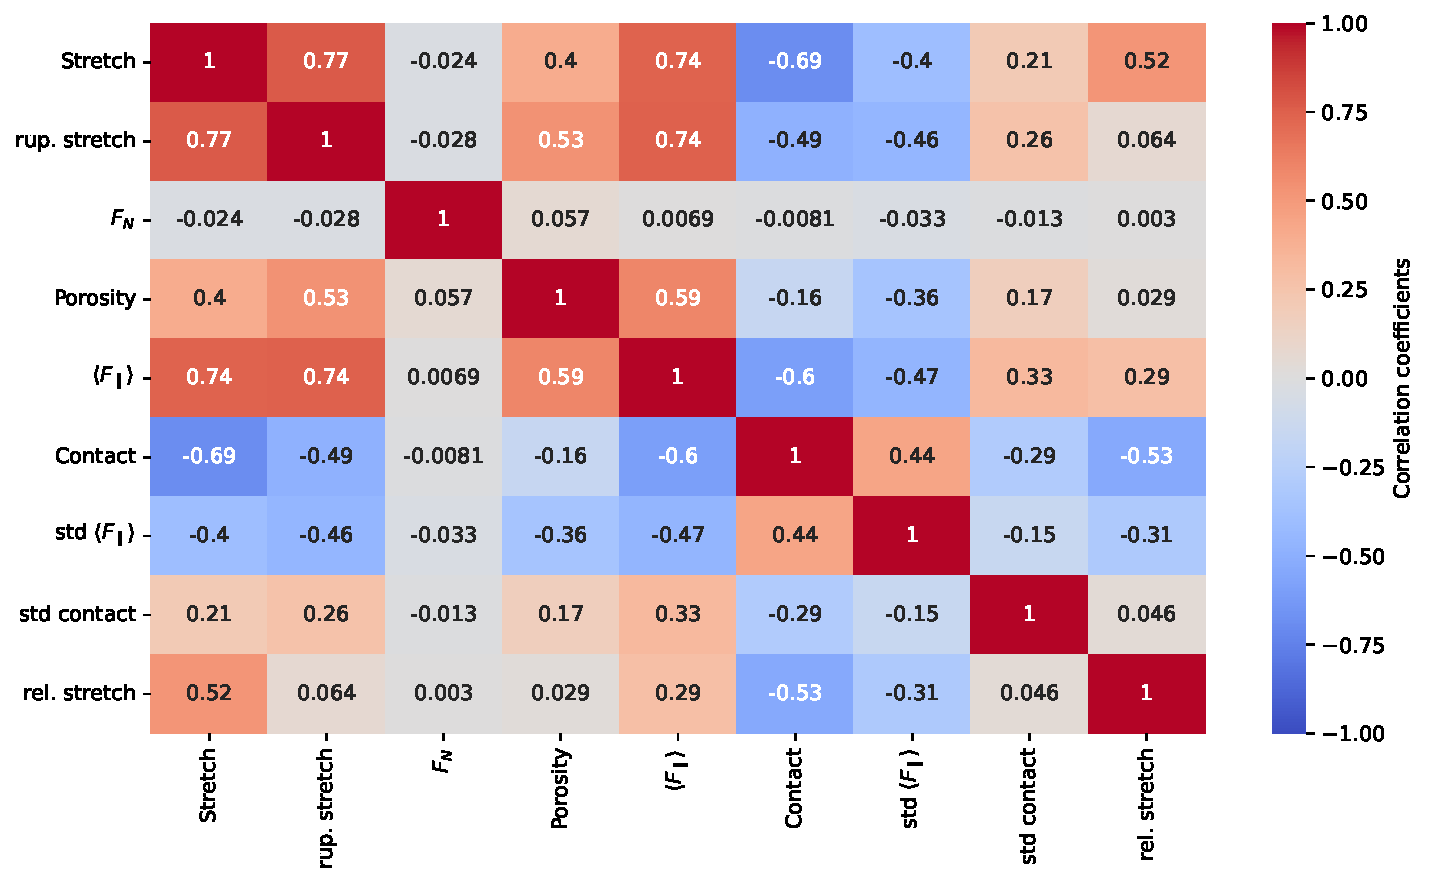
\includegraphics[width=\linewidth]{figures/ML/corrcoef_matrix.pdf}
  \caption{Pearson product-moment correlation coefficients for the full datset (see \cref{tab:dataset_summary}).}
  \label{fig:corrcoef_matrix}
\end{figure}

From \cref{fig:corrcoef_matrix} we especially notice that the mean
friction force $\langle F_{\parallel} \rangle$ has a signifciant positively
correlation with stretch $(0.77)$ and porosity $(0.60)$ (void fraction).
However, the relative stretch, which is scaled by the rupture stretch, has a
weaker correlation of only 0.25 which indicates that it is the absolute stretch
value that has the most significant impact on the friction force increase during
stretching. This is further supported by the fact that the mean friction and the
rupture stretch is also strongly positively correlated $(0.78)$. From figure
\cref{fig:corrcoef_matrix} we also observe that the contact bond count is
negatively correlated with the mean friction $(-0.67)$ and the stretch value
$(-0.74)$ which is consistent with the trend observed in the pilot study  \cref{fig:multi_stretch_contact} and \cref{fig:multi_stretch_mean_fric}) of the
contact decreasing with increasing stretch and mean friction. However, we must
take note that the correlation coefficients is a measure of the strength and slope of a
forced linear fit on the data. We clearly observed a non-linear relationship between stretch and mean friction for the tetrahedron and honeycomb pattern used in the pilot study  \cref{fig:multi_stretch_mean_fric}) where the relationship was partwise characterized by a postive correlation for some stretch ranges and partwise negative correlation for other stretch ranges. Hence, interesting strong regime-specific correlations might not be accurately highlighted by the correlation coefficients shown in \cref{fig:corrcoef_matrix}.

In \cref{fig:corr_vis} we have visualized the data (excluding the pilot study) for chosen pairs of variables on the axes. In addition to a visual confirmation of how the given correlations look in a 2D plot we also get a feeling for the coverage in various areas of the parameter space that we are eventually going to feed the neural network. The honeycomb pattern is spanning a significant larger range of stretch, contact and mean friction makes the data rather biased towards the Honeycomb pattern in thoose areas. 
% Judging form the combinned information of the pilot study and the data distribution shown in \cref{fig:corr_vis} it would not be surprising if the machine learning were to learn that the honeycomb pattern is superiour for 

Uncommented to decrease loading time
\begin{figure}[H]
  \centering
  \begin{subfigure}[t]{0.49\textwidth}
      \centering
      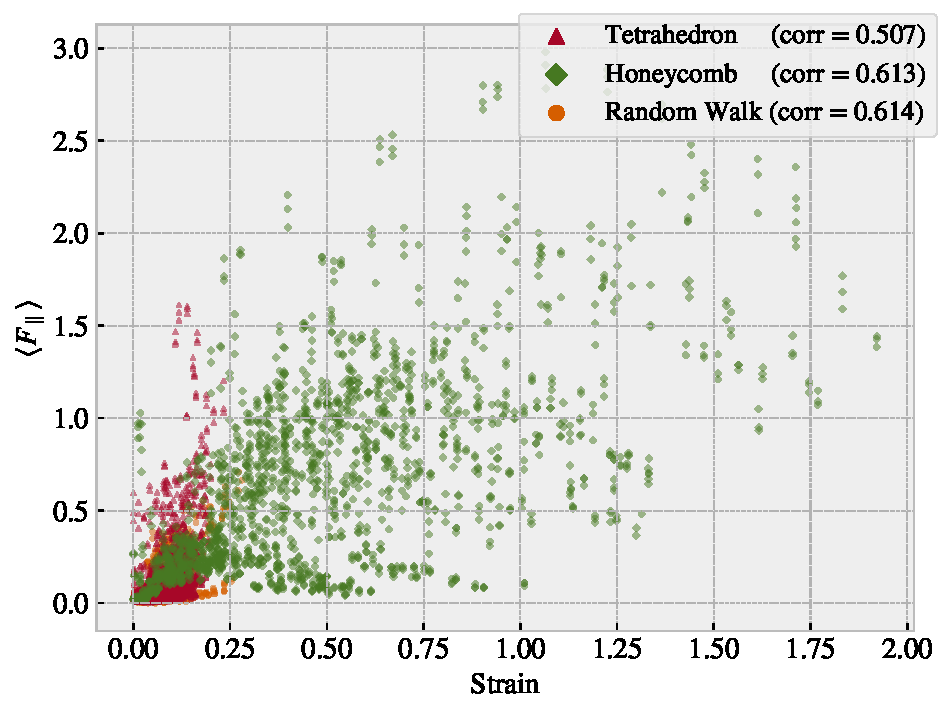
\includegraphics[width=\textwidth]{figures/ML/corr_stretch_Ff.pdf}
      \caption{}
      % \label{fig:}
  \end{subfigure}
  \hfill
  \begin{subfigure}[t]{0.49\textwidth}
      \centering
      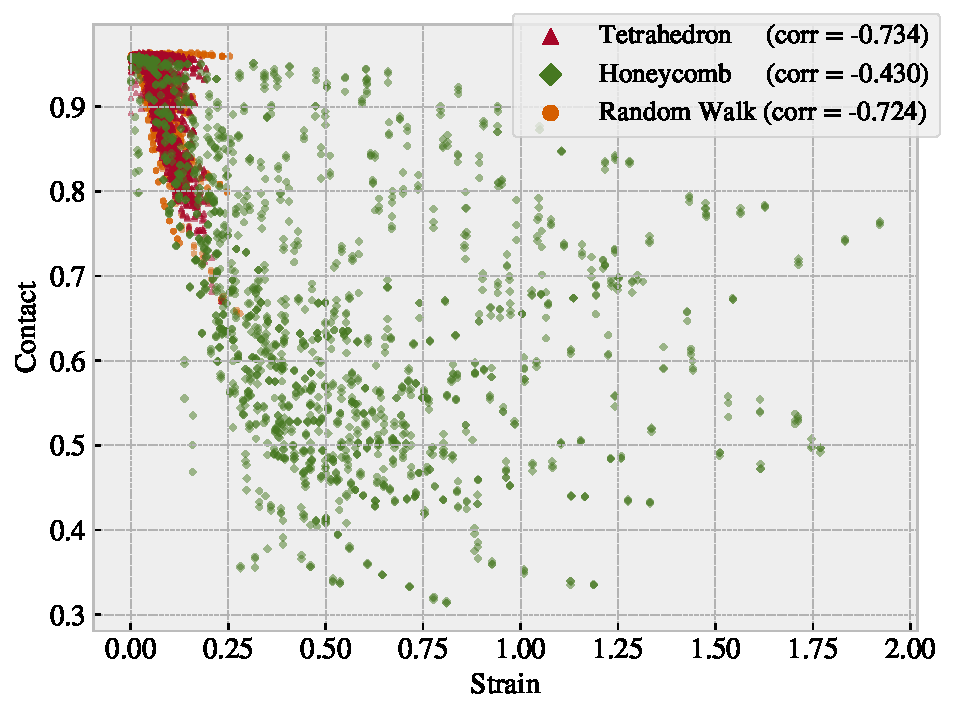
\includegraphics[width=\textwidth]{figures/ML/corr_stretch_contact.pdf}
      \caption{}
      % \label{fig:}
  \end{subfigure}
  \hfill
  \begin{subfigure}[t]{0.49\textwidth}
      \centering
      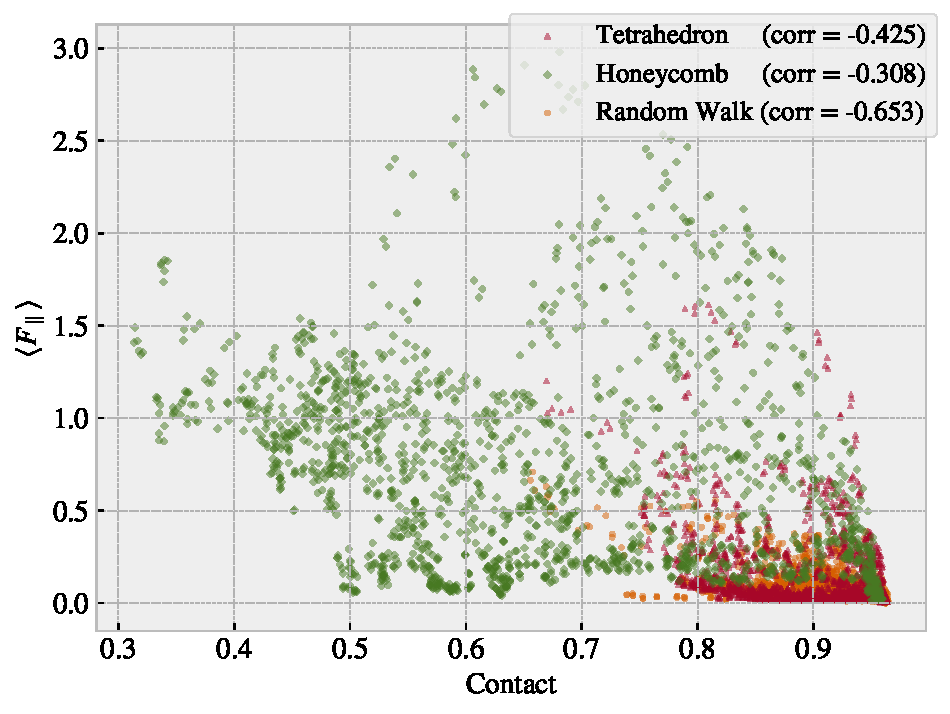
\includegraphics[width=\textwidth]{figures/ML/corr_contact_Ff.pdf}
      \caption{}
      % \label{fig:}
  \end{subfigure}
  \hfill
  \begin{subfigure}[t]{0.49\textwidth}
      \centering
      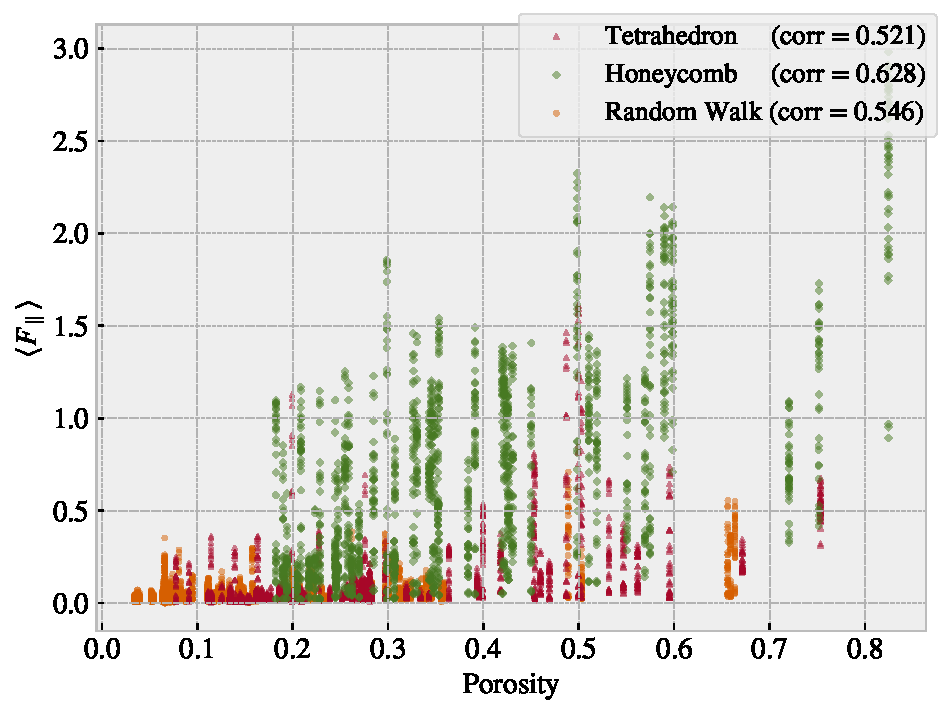
\includegraphics[width=\textwidth]{figures/ML/corr_porosity_Ff.pdf}
      \caption{}
      % \label{fig:}
  \end{subfigure}
  \hfill
     \caption{Scatter plot of the data sets Tetrahedron, Honeycomb and Random Walk (excluding the pilot study) for various variable combinations in order to visualize some chosen  correlations of interest and distributions in the data}
     \label{fig:corr_vis}
\end{figure}


\section{Properties of interest} 
From the Pilot study we discovered that it might be possible to achieve a negative friction coefficient for certain kirigami cut configurations under the assumption of a system with coupled normal force $F_N$ and stretch $S$. This stands as the main property of interest to explore further in the dataset. However, it is not obvious how one should quanity this in a rigorous manner. The friction coefficient is by our definition (\hl{see theory sec XXX}) given as the slope of the friction vs.\ normal force curve. For two data points $(F_{N,1}, F_{f,1}), (F_{N,2}, F_{f,2})$, $F_{N,1} < F_{N,2}$ we would evaluate the associated friction coefficient $\mu_{1,2}$ as 
\begin{align*}
  \mu_{1,2} = \frac{F_{f,2} - F_{f,1}}{F_{N,2} - F_{N,1}} = \frac{\Delta F_f}{\Delta F_N}
\end{align*}
In the pilot study it became clear that the effects on friction under the change of $F_N$ is neglible in comparison to the effects under change of $S$. Thus, by working under the assumption $F(F_N, S) \sim F(S)$ and a coupling $F_N \propto R\cdot S$ with coupling ratio $R$ we get 
\begin{align}
  \mu_{1,2}(S_1, S_2) = \frac{\Delta F_{f}(S_1, S_2)}{R(S_2 - S_1)} \propto \frac{\Delta F_{f}(S_1, S_2)}{\Delta S},
  \label{eq:mu_stretch}
\end{align}
With the above reasoning we have in practive exchanged $F_N$ with $S$ in the
expression for the friction coefficient. This means that we are interested in  a
negative slope on the friction vs.\ stretch curve which corresponds to a
negative friction coefficient in our proposed coupled system. The next question
remaining is then how to evaluate the strength of this property. By definition,
the minimum slope value would give the lowest friction coefficient. However, for two data points with a small $\Delta S$, corresponding to small denominator in \cref{eq:mu_stretch}, would potentially result in big $|\mu|$ without any signifiant decrease in friction. Hence, we choose to consider the drop in friction with increasing stretch. For a discrete dataset we can locate all local maxima and evaluate the difference to all succeeding local minema. The biggest drop will serve as our indicator for a signifcant negative friction coefficient. In this evaluation we do not guarantee a monotonic decrease of friciton in the range of the biggest drop, but when seearching among multiple configurations this is considered a descent strategy to highlight configurations of interest worthy of further investigation. 

In addition to the biggest drop in friction we also look at minimum abnd maximum friction along with the difference between theese extrema. In \cref{tab:data_properties} we summarized the extrema of these properties. The corresponding friction vs.\ stretch profiles and configurations are visualized for each property category in \crefrange{fig:PP_min}{fig:PP_max_drop}. The stretch profiles for all the configurations are shown in appendix \cref{sec:data_stretch_profiles}.


\begin{table}[H]
  \begin{center}
  \caption{Evaluation of the properties of interest for our dataset.}
  \label{tab:data_properties}
  \begin{tabular}{| c | c | c | c|} \hline
  \textbf{Tetrahedron} & Configuration & Stretch & Value [nN]  \\ \hline
  Min $F_{\text{fric}}$ & $(3,9,4)$ &  0.0296 & 0.0067 \\ \hline
  Max $F_{\text{fric}}$ & $(5,3,1)$ & 0.1391 & 1.5875 \\ \hline
  Max $\Delta F_{\text{fric}}$  & $(5, 3, 1)$ & $[0.0239, 0.1391]$ & 1.5529 \\ \hline
  Max drop & $(5,3,1)$ & $[0.1391, 0.1999]$ & 0.8841 \\ \hline
  \multicolumn{4}{c}{} \\ \hline
  % \textbf{Tetrahedron} & \multicolumn{3}{c|}{} \\ \hline
  \textbf{Honeycomb} & Configuration & Stretch & Value [nN]  \\ \hline
  Min $F_{\text{fric}}$ & $(2, 5, 1, 1)$ &  0.0267 & 0.0177 \\ \hline
  Max $F_{\text{fric}}$ & $(2, 1, 1, 1)$ & 1.0654 & 2.8903 \\ \hline
  Max $\Delta F_{\text{fric}}$  & $(2, 1, 5, 3)$ & $[0.0856, 1.4760]$ & 2.0234 \\ \hline
  Max drop & $(2, 3, 3, 3)$ & $[0.5410, 1.0100]$ & 1.2785 \\ \hline
  \multicolumn{4}{c}{} \\ \hline
  \textbf{Random walk} & Configuration & Stretch & Value [nN]  \\ \hline
  Min $F_{\text{fric}}$ & 12 &  0.0562 & 0.0024\\ \hline
  Max $F_{\text{fric}}$ & 96 & 0.2375 & 0.5758 \\ \hline
  Max $\Delta F_{\text{fric}}$  & 96 & $[0.0364, 0.2375]$ & 0.5448 \\ \hline
  Max drop & 01 & $[0.0592, 0.1127]$ & 0.1818 \\ \hline
\end{tabular}
\end{center}
\end{table}
% Popup
% ['(3, 9, 4)', 0.0296407442523106, 0.006738434728040425]
% ['(5, 3, 1)', 0.139120019152679, 1.5874991413277917]
% ['(5, 3, 1)', 0.0238700191526787, 0.139120019152679, 1.5529155085058322]
% ['(5, 3, 1)', 0.139120019152679, 0.199920019152683, 0.8840614643066859]

% Honeycomb
% ['(2, 5, 1, 1)', 0.0267215709876031, 0.01771035812444661]
% ['(2, 1, 1, 1)', 1.06536290170726, 2.8903313732271183]
% ['(2, 1, 5, 3)', 0.085589883539189, 1.47601988353919, 2.023377918411005]
% ['(2, 3, 3, 3)', 0.541004661720013, 1.01001466172002, 1.278541503443495]

% RW
% ['12', 0.0562087686350666, 0.002350782025058632]
% ['96', 0.237523191134115, 0.5757864994802119]
% ['96', 0.0363631911341175, 0.237523191134115, 0.5447910475168634]
% ['01', 0.0591598822685843, 0.112739882268582, 0.18175926264779968]

\begin{figure}[H]
  \centering
  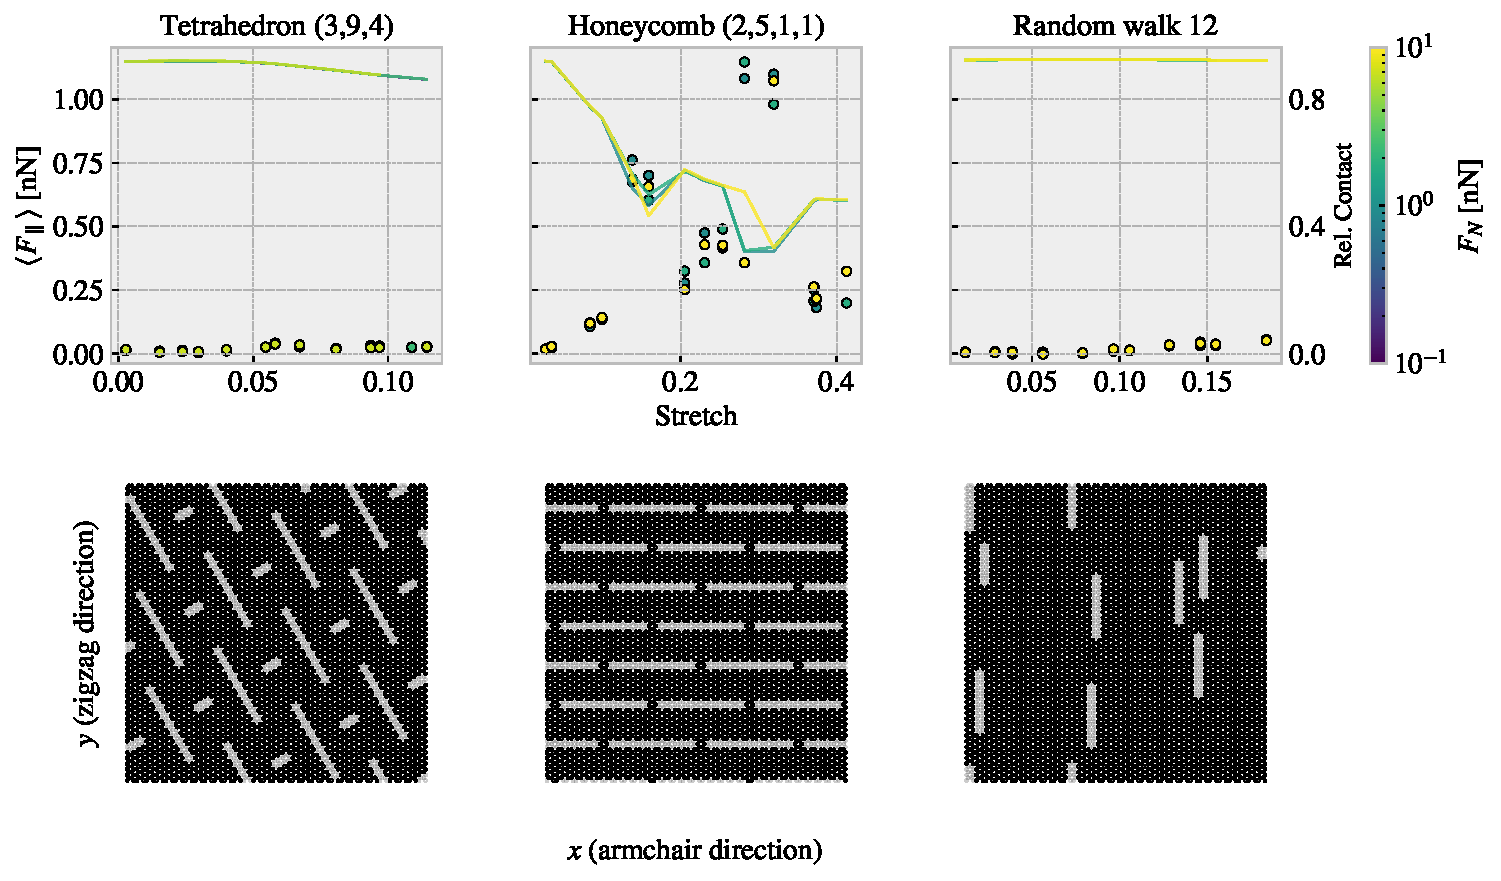
\includegraphics[width=\linewidth]{figures/stretch_profiles/PP_min.pdf}
  \caption{Minimum friction: Configurations corresponding to the minimum friction.}
  \label{fig:PP_min}
\end{figure}


\begin{figure}[H]
  \centering
  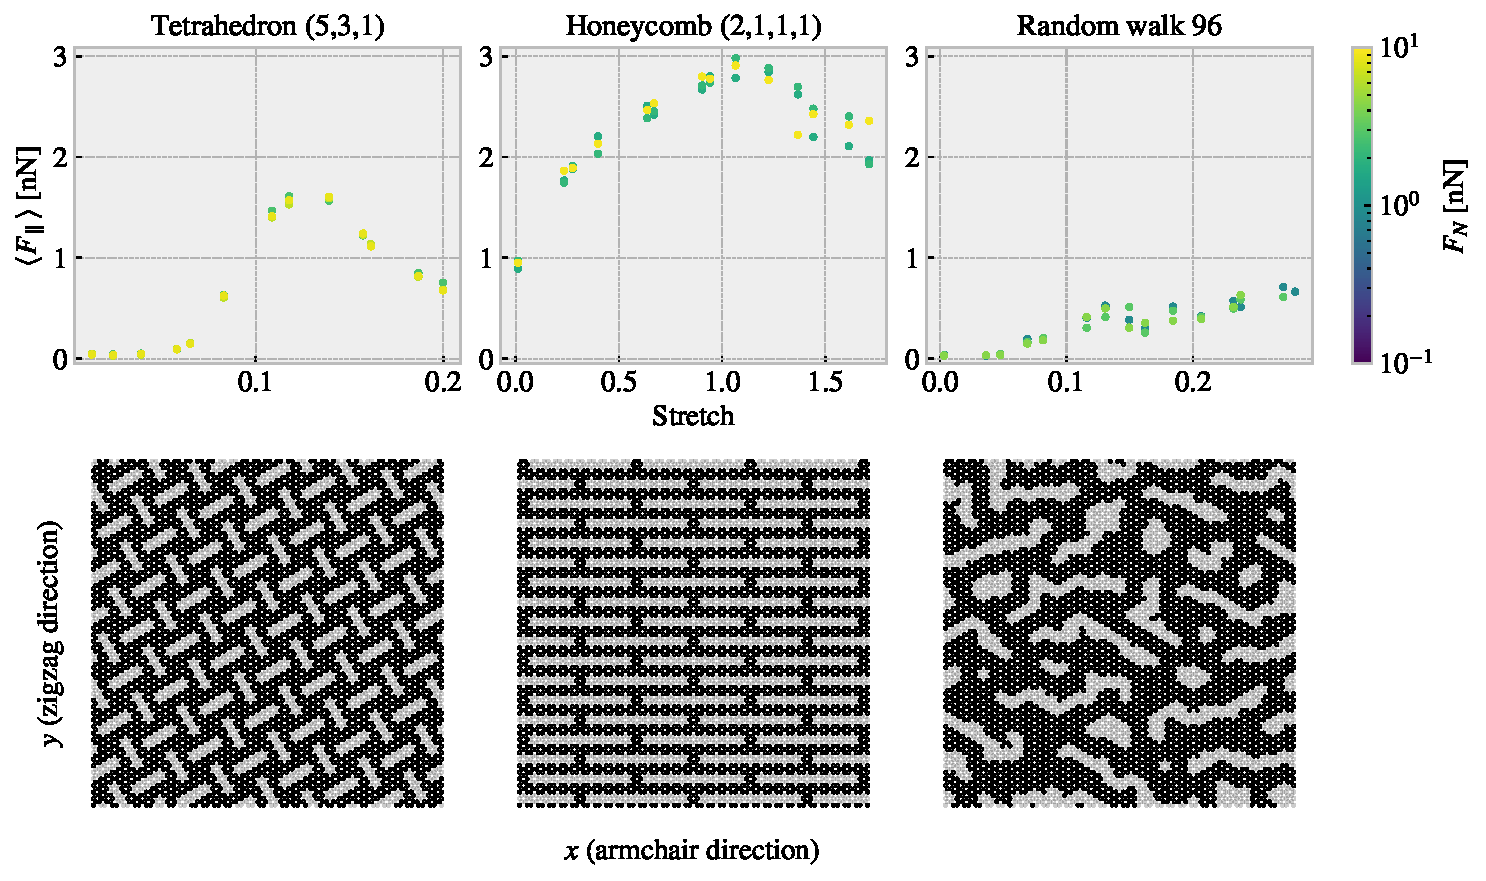
\includegraphics[width=\linewidth]{figures/stretch_profiles/PP_max.pdf}
  \caption{Maximum friction: Configurations corresponding to the maximum friction.}
  \label{fig:PP_max}
\end{figure}


\begin{figure}[H]
  \centering
  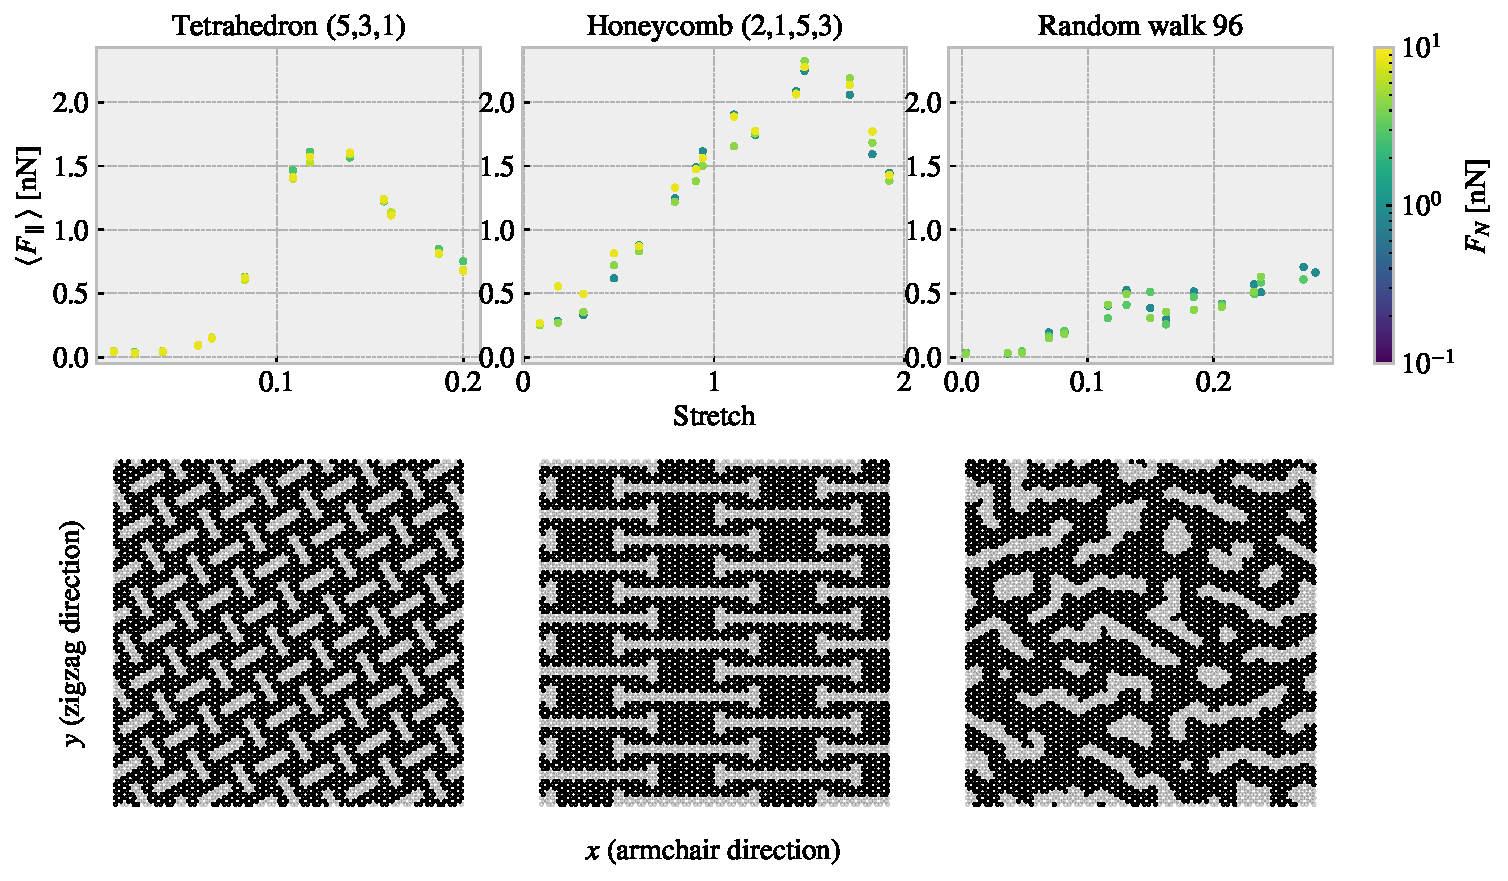
\includegraphics[width=\linewidth]{figures/stretch_profiles/PP_max_diff.pdf}
  \caption{Maximum Difference: Configurations corresponding to the biggest difference in friction in the dataset for each pattern.}
  \label{fig:PP_max_diff}
\end{figure}  

\begin{figure}[H]
  \centering
  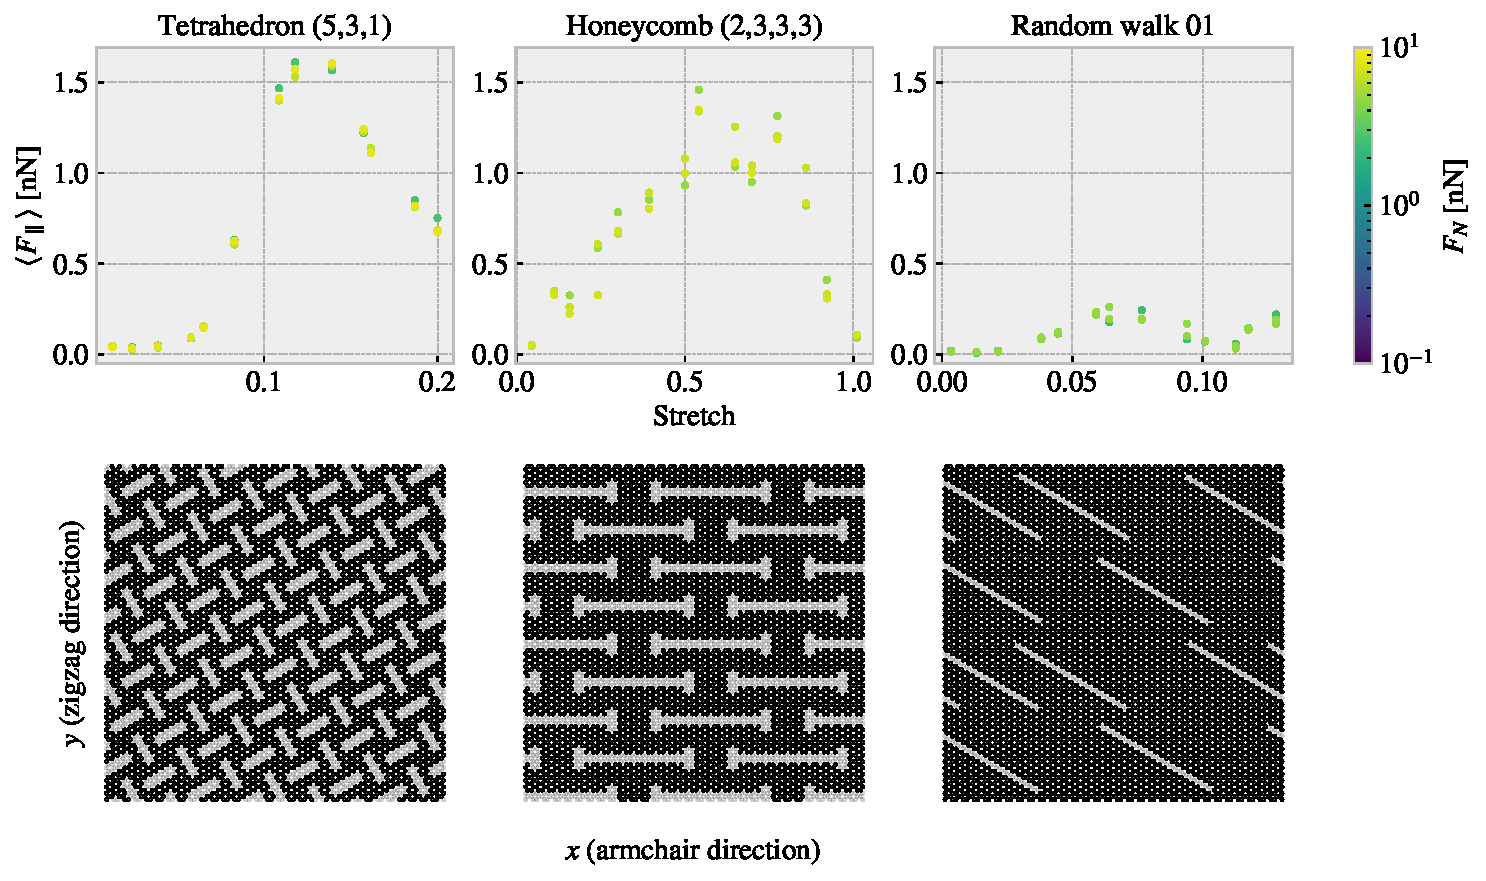
\includegraphics[width=\linewidth]{figures/stretch_profiles/PP_max_drop.pdf}
  \caption{Maximum drop: Configuratiosn corresponding to the biggest friction drop in the dataset for each pattern.}
  \label{fig:PP_max_drop}
\end{figure}  





% \begin{figure}[H]
%   \centering
%   \begin{subfigure}[t]{0.49\textwidth}
%       \centering
%       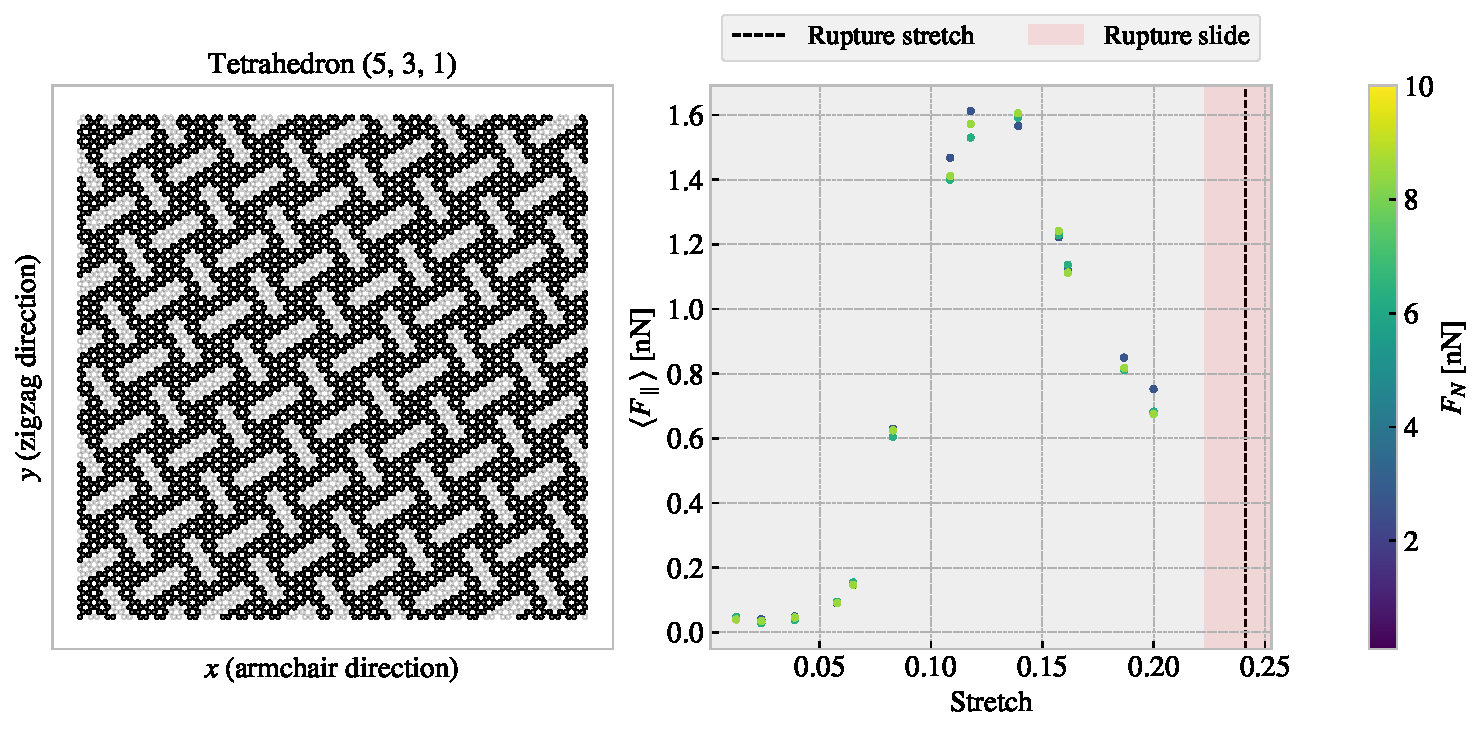
\includegraphics[width=\textwidth]{figures/stretch_profiles/PP_pop_27.pdf}
%       \caption{}
%   \end{subfigure}
%   \hfill
%   \begin{subfigure}[t]{0.49\textwidth}
%       \centering
%       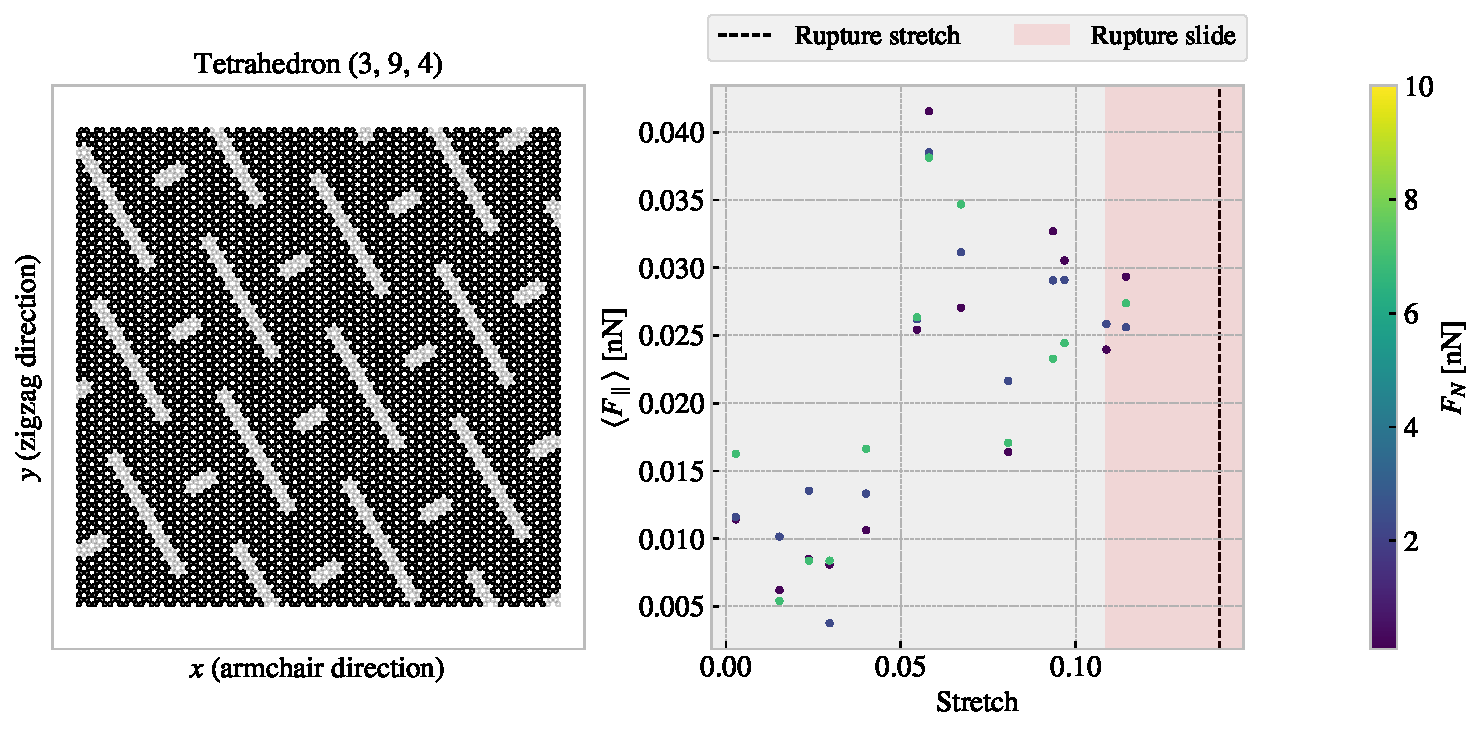
\includegraphics[width=\textwidth]{figures/stretch_profiles/PP_pop_31.pdf}
%       \caption{}
%   \end{subfigure}
%   \hfill
%   \begin{subfigure}[t]{0.49\textwidth}
%       \centering
%       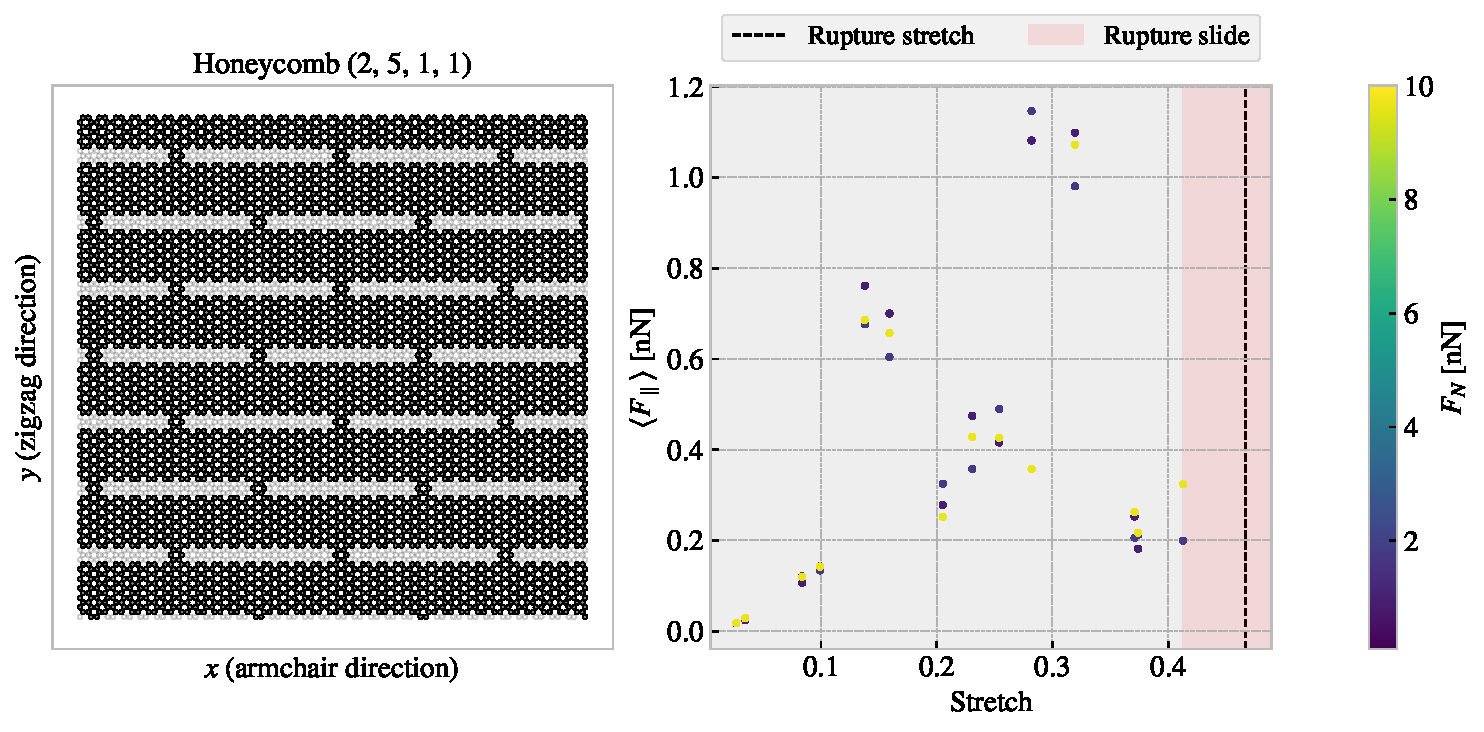
\includegraphics[width=\textwidth]{figures/stretch_profiles/PP_hon_6.pdf}
%       \caption{}
%   \end{subfigure}
%   \hfill
%   \begin{subfigure}[t]{0.49\textwidth}
%       \centering
%       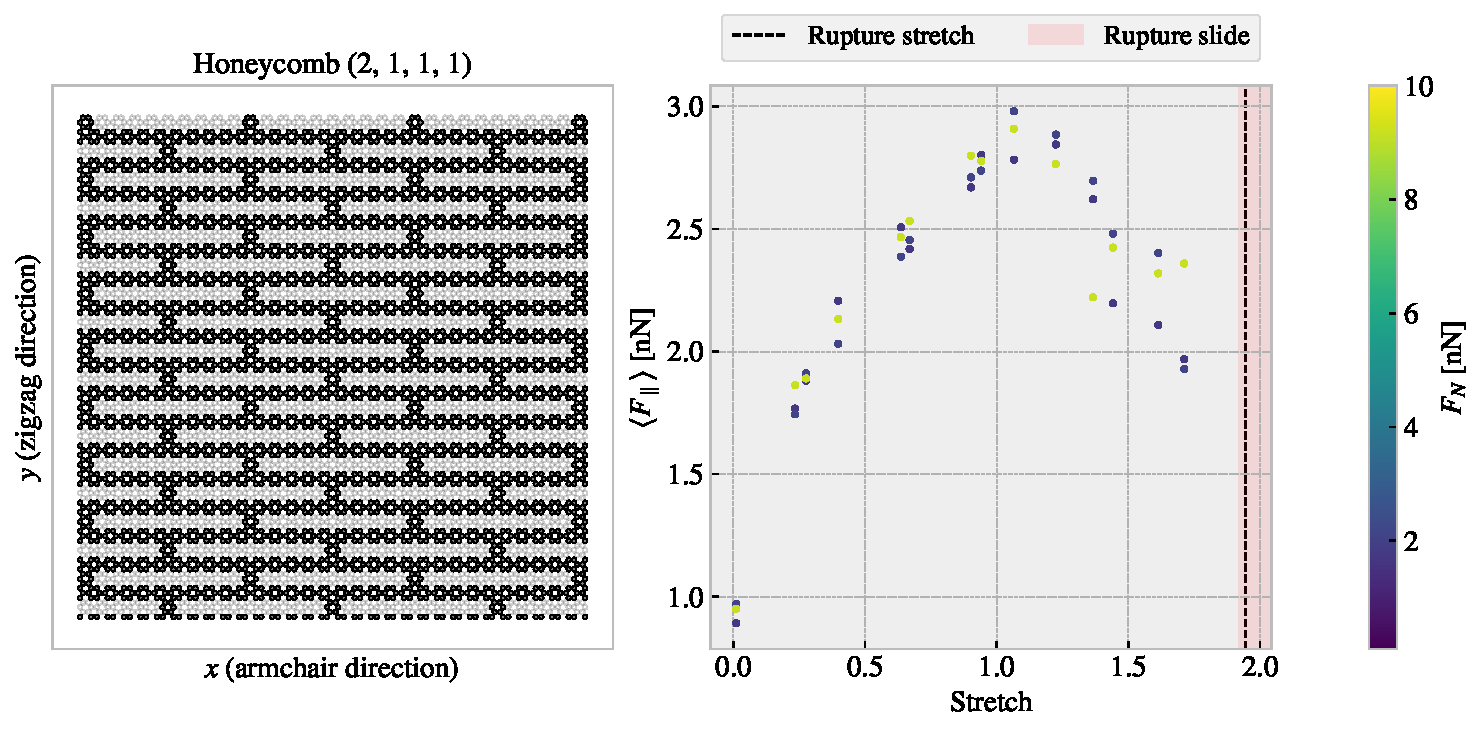
\includegraphics[width=\textwidth]{figures/stretch_profiles/PP_hon_12.pdf}
%       \caption{}
%   \end{subfigure}
%   \hfill
%   \begin{subfigure}[t]{0.49\textwidth}
%       \centering
%       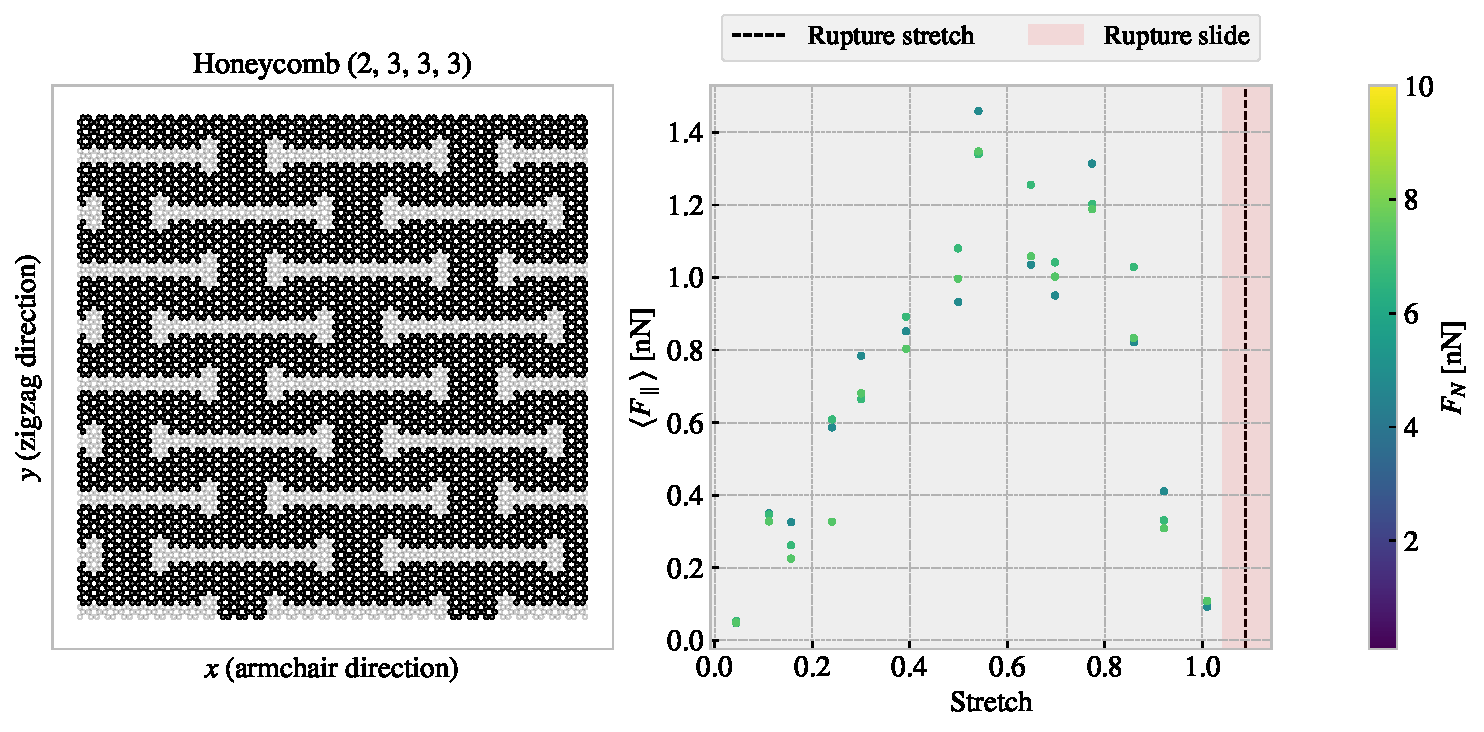
\includegraphics[width=\textwidth]{figures/stretch_profiles/PP_hon_28}
%       \caption{}
%   \end{subfigure}
%   \hfill
%   \begin{subfigure}[t]{0.49\textwidth}
%       \centering
%       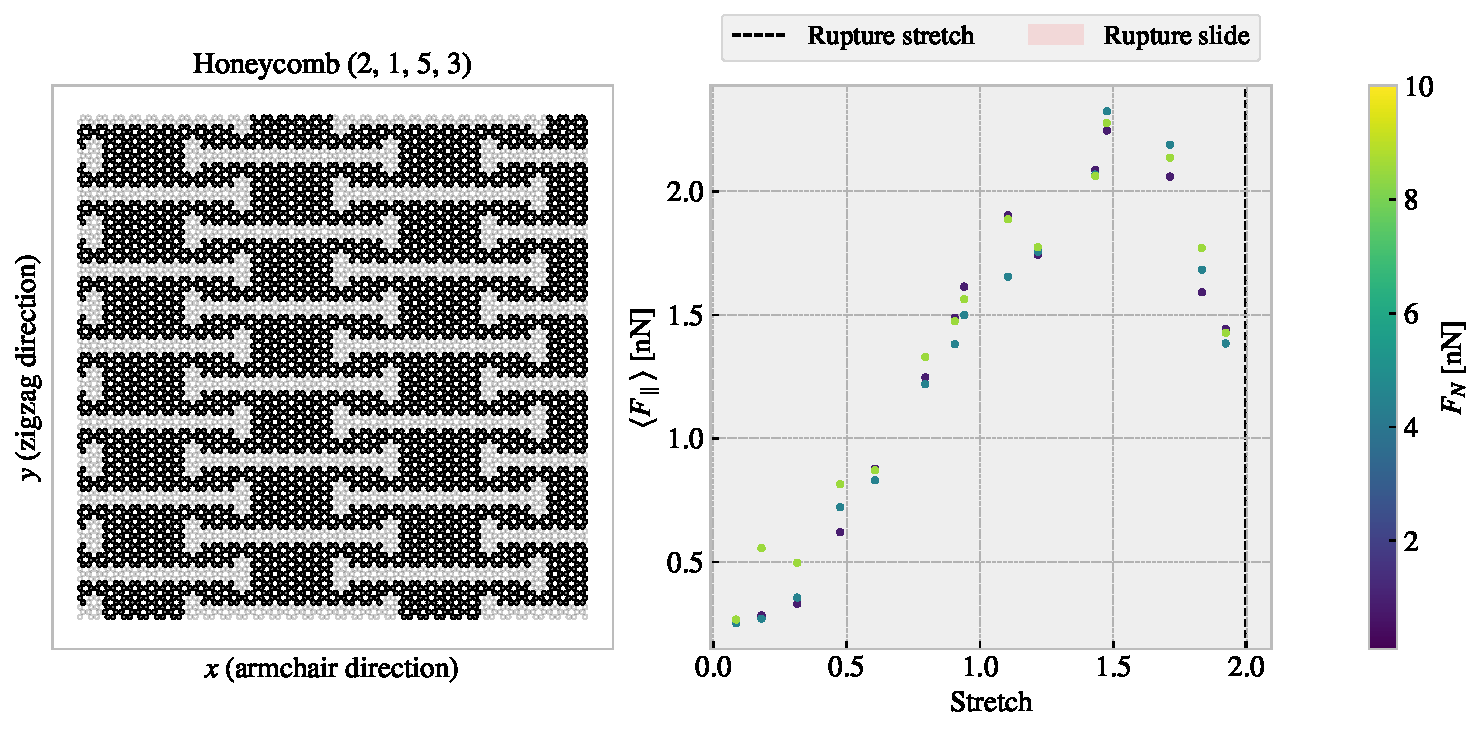
\includegraphics[width=\textwidth]{figures/stretch_profiles/PP_hon_42.pdf}
%       \caption{}
%   \end{subfigure}
%   \hfill
%   \begin{subfigure}[t]{0.49\textwidth}
%       \centering
%       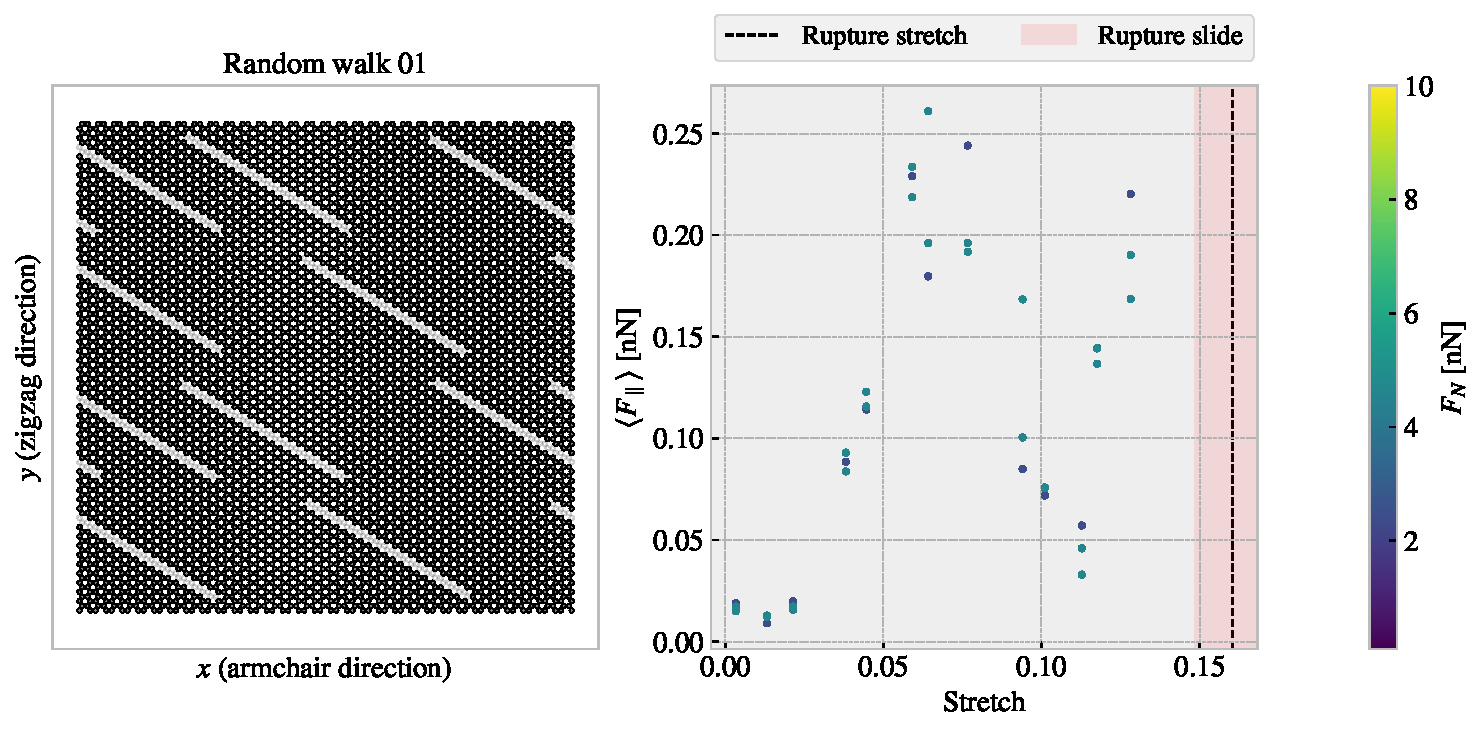
\includegraphics[width=\textwidth]{figures/stretch_profiles/PP_RW01.pdf}
%       \caption{}
%   \end{subfigure}
%   \hfill
%   \begin{subfigure}[t]{0.49\textwidth}
%       \centering
%       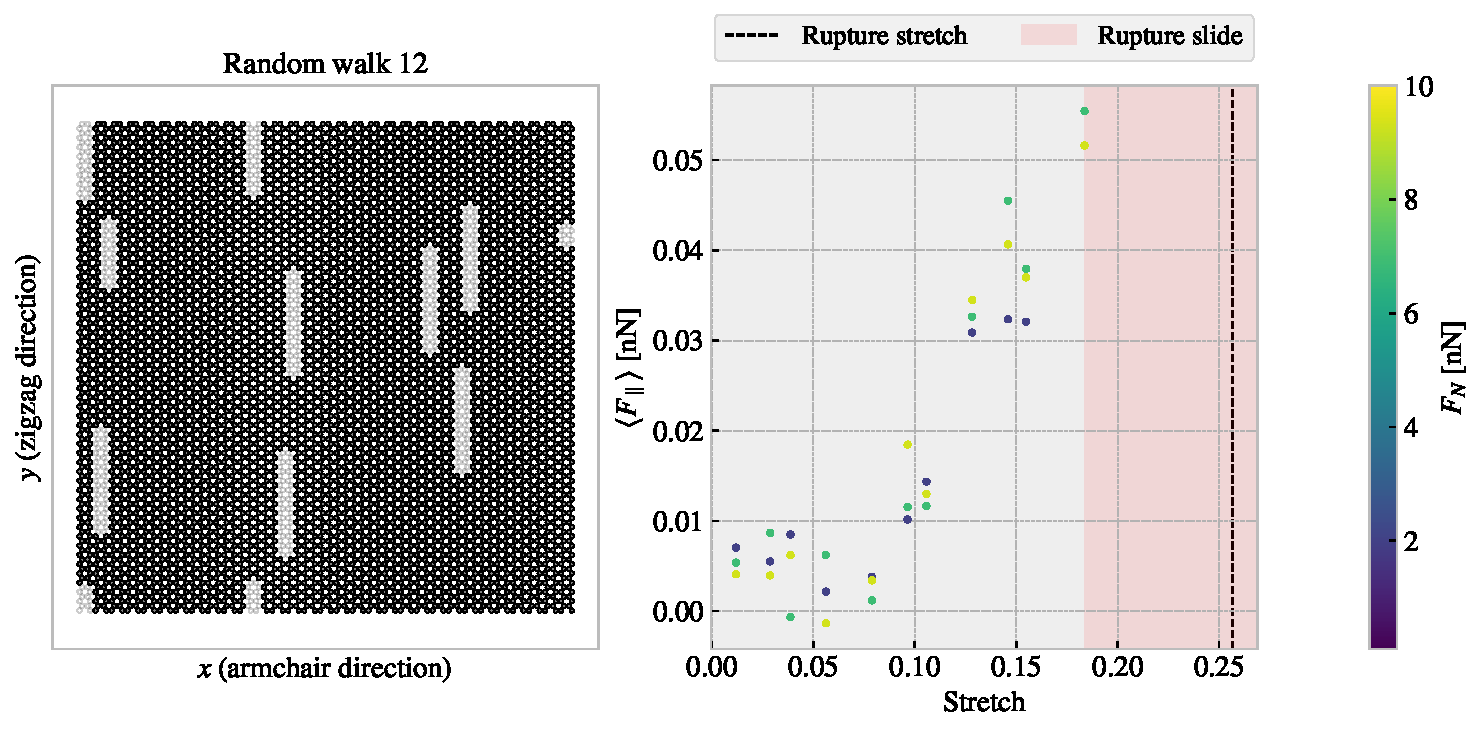
\includegraphics[width=\textwidth]{figures/stretch_profiles/PP_RW12.pdf}
%       \caption{}
%   \end{subfigure}
%   \hfill
%   \begin{subfigure}[t]{0.49\textwidth}
%       \centering
%       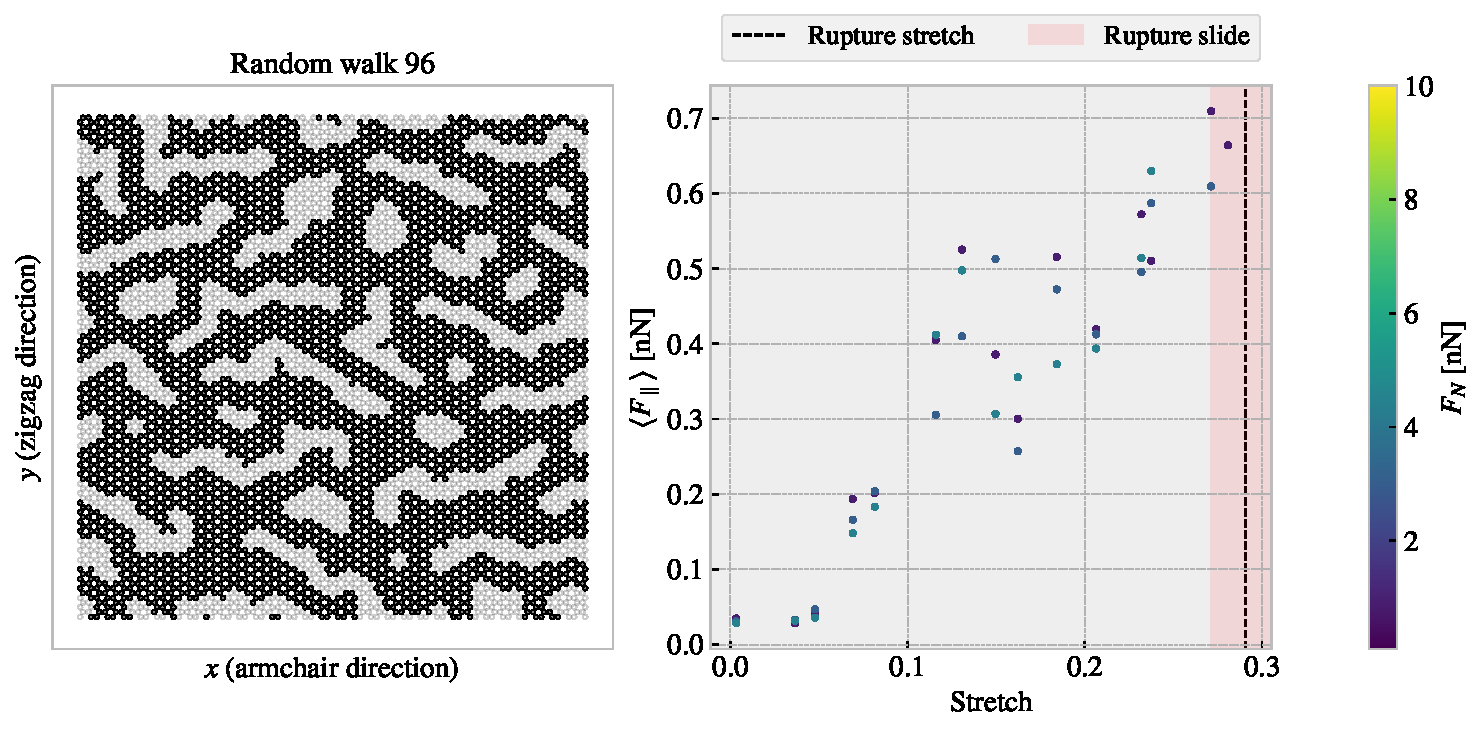
\includegraphics[width=\textwidth]{figures/stretch_profiles/PP_RW96.pdf}
%       \caption{}
%   \end{subfigure}
%   \hfill
%      \caption{}
%      \label{fig:}
% \end{figure}








\section{Machine learning}

General stuff to include. Remember to talk about batchnorm, optimizer, stopping at best epoch. 


\subsection{Architecture}
Due to the spatial dependencies in the kirigami configurations we use a convolutional neural network (\acrshort{CNN}). Studies on similar a similar system envolving the graphene sheet have used a VGGNet style of network, Hanakata et al.\ \cite{PhysRevLett.121.255304}\cite{PhysRevResearch.2.042006} and Wan et al.\ \cite{graphene/hBN}, which we adopt for this study as well. The VGGNet-16 architecture illustrated in \cref{fig:VGGNet16} shows the key features; 
\begin{itemize}
  \item The image is processed through a series of $3 \times 3$ convolutional filters (the smallest size to capture spatial dependencies) using a stride of 1 with an increasing number of channels throughout the network. Each convolutional layer is followed by a ReLU acitivation. 
  \item The spatial dimensions are reduced by a max pooling ($2 \times 2$, stride of 2), which half the spatial resolution each time. 
  \item The latter part of the network consist of fully connected part followed by a ReLU activation. The image is first processed in a $1 \times 1$ which performs a linear mapping to a series of fully connected layers. 
\end{itemize}

\begin{figure}[H]
  \centering
  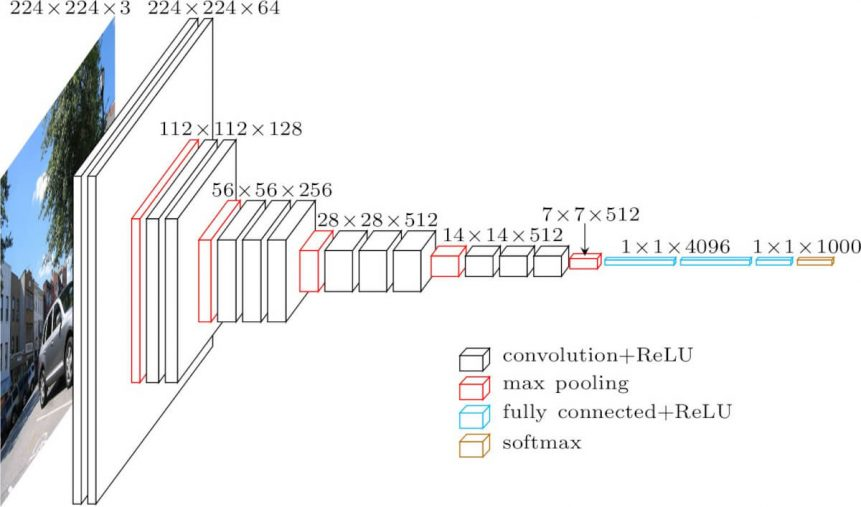
\includegraphics[width=0.7\linewidth]{figures/ML/VGGNet16.jpg}
  \caption{VGGNet 16. Source \url{https://neurohive.io/en/popular-networks/vgg16/}.}
  \label{fig:VGGNet16}
\end{figure}

In contrast to the VGGNet-16 we restrict ourselves to building the convolutional part in terms of blocks of (convolution, ReLU, max pooling), thus not allowing for any connsecutive convolutional filters without performing a max pooling as well. The fully connected blocks is defined as (fully connected, ReLU) similar to that of the VGGNet model. Hanakata et al.\ and Wan et al.\ used a similar construction before settling on the models
\begin{align*}
  \text{Hanakata et al.\ \cite{PhysRevLett.121.255304}} & \qquad C16 \ C32 \ C64 \ D64, \\ 
  \text{Wan et al.\ \cite{graphene/hBN}} & \qquad C16 \ C32 \ D32 \ D16,
\end{align*}
Where $C$ denotes a convolutional block with the following number being the number of channels and $D$ a fully conneted (dense) layer with the number denoting number of nodes. For the process of determing a suiting complexity for the architecture we adpot the approach by Wan et al.\ \cite{graphene/hBN} who used a ``staircase'' pattern for combinning convolutional and fully connected blocks. By defining a starting number of channels $S$ and network depth $D$ we fill the first half with convoliutional blocks doubling in channel number for each layer and the latter half with fully connected blocks starting setting the number of nodes as the reverse pattern used for the number of channels. Following this pattern a $(S=4, D=8)$ would take the form
\begin{align*}
  \text{Input} \to \underbrace{\overbrace{C4}^{S \ = \ 4}C8 \ C16 \ C32 \ D32 \ D16 \ D8 \ D4}_{D \ = \ 8} \to \text{Output}.
\end{align*} 
This provides a simple description where $S$ and $S$ and can be varied systematically for a grid search over architecture complexity. 


% We also throw in a batchnorm!

\subsection{Data handling}
\subsubsection{Input}
We use three variables as input: Kirigami configuration, stretch of the sheet
and applied normal load. While the first is a two-dimensional input the latter
are both scalar values. This gives rise to two main options for the data structure
\begin{enumerate}
  \item Expand the scalar values (stretch and load) into 2D matrices of the same
  size as the kirigami configuration by copying the scaler value to all positions. This can then be merged into an image of three channels used as a single input.  
  \item Pass only the kirigami configuration through the \acrshort{CNN} part of the network and introduce the remaining scalar values into the \acrshort{FC} part of the network. 
\end{enumerate}
Both options utilize the same data, but the first emphasizes that the configurations should be processed in relation to the applied stretch and load, while the latter represent a more independent processing. We implemented the option to do both variations, but it quickly became clear that option 1 was producing the most promising result ({hl{do more rigorous presentation of this?}}).

\subsubsection{Output}
For the output we are mainly concerned about the mean friction and the rupture
detection. In combination this make us able to produce a friction vs.\ stretch curve with an estimated stopping point as well.  However, it has often been proven useful to introduce more variables in the output in order to strengthen the network training
(\hl{get source}). In addition, this gives us more options for exploring the
relationship in the data later on. Therefore, we include maximum friction, contact
count, porosity and rupture stretch in the output as well. Notice that rupture stretch
refers to the value found in the rupture test without load, but as the sheet
always ruptures before or just around this point in a loaded state this provides
some information for the training to lean on, even though it is in the output
state. In principle, we could add a penalty whenever the network predicts the
sheet to be attatched for stretch values above the rupture stretch, but we found
the performance of the rupture prediction to be satisficatory without such penalties. Notice that we weight the importance of these
variables differently as explained in the section regarding the loss. 

\subsubsection{Data augmentation}
In order to increase the ulility of the limited data availble, one can introduce data augmentation. For classification task this includes distortions such as color shift, zoom, flip etc. However, such distorions are only valid since the classification network should still classify a cat as a cat even though it is suddenly a bit brigther or flipped upside down. For our problem we can only use augmentation that matches a physical symmetry. Such a symmetry exist only for relfection accross the y-axis. We cannot do this across the
x-axis as the sheet is translated in a positive y-direction meaning that the reflected version would not be sliding backwards for which we do not expect to be symmetric in results. We definitely expect a snow plow to perform differently when attached in reverse and thus by analogy we would expect the direction of sliding with respect to the configuration to be of importance. 

\subsection{Loss}
The output contain two different types of variables: scalar values and binaray values (0: False 1: True)

For the scalar values we use the Mean Squared Error (\acrshort{MSE})
\begin{align*}
  L_{\text{MSE}} = \frac{1}{N} \sum_{i = 1}^N (y_i - \hat{y}_i)^2,
\end{align*}
where $N$ is the number of data entries and $y$ are the true variables and
$\hat{y}$ are the predicted values. For the binary output we use binary cross entropy 
\begin{align*}
  L_{\text{BCE}} = -\frac{1}{N} \left[\sum_{i = 1}^N [t_i\log{(p_i)} + (1-t_i)\log{(1 - p_i)}]\right],
\end{align*}
where $t\in \{0,1\}$ is the truth label. \hl{Does this belong in theory
entirely?}. We calculate the total loss as a weighted sum between the loss associated with
each variable
\begin{align*}
  L_{tot} = \sum_{v} W_v\cdot L_v.
\end{align*}
We choose the weights to be $1/2$ for the mean friction and $1/10$ for the
remaining 5 variables thus sharing evenly for the remaining 50\% of the weight. During the introductionary phase of the training we tried varying these weights,
but we found that the results varied little and concluded that the training is not very sensitive to this choice, and disregarded further tuning of this parameter. 

\subsection{Hypertuning}
% Overfitting
For the hypertuning of \acrshort{ML} parameters we focus on architecture complexity, learning rate, momentum and weight decay. We train with the adam optimizer with the default values of $beta_1 = 0.9, \beta_2 = 0.999$ and zero weight decay. For the batch size we use 32 for training and 64 for validation. We train the network for a maximum of 1000 epochs, but we save the best model during training based on lowest validation loss. Since the learning rate is considered to be one of the most important hyperparameters we will determine a suitable choice for the learning individually throughout the two major grid searches:
\begin{enumerate}
  \item Architecture complexity grid search of $S$ vs.\ $D$ with individually chosen learning rates for each complexity combination.
  \item Momentum vs.\ weight decay grid search with learning range chosen with regard to the momentum setting. 
\end{enumerate}
We consider first the architectures in the range $S \times D =
\{2,4,8,16,32,64,128,256\} \times \{4,6,8,10,12,14\}$. For each architecture
complexity we perform an initial learning rate range test, increaing the
learning rate for each batch iteration until the training loss diverges. the suggested learning rate is then determined as the point for which the training loss decreases most rapidly. The learning rate is increased exponentially from \num{e-7} to 10 with increments for each training batch iteration. This is done for just a single epoch where a training batch size of 32 yields a total of 242 batches in the training data. This corresponds to an exponent increment of approximately $1/30$ giving a relative increase $10^{1/30} \sim 108\%$ per batch iteration. The learning rate range test is presented in \cref{fig:LR_range}. We notice that the suggested learning rate decreases with increasing number of model parameters. This decrease is further independent on the specific relationship between $S$ and $D$. % Looks a bit like power functions, but I do not really think this is important to say since it is not backed by a fit. 

\begin{figure}[H]
  \centering
  \begin{subfigure}[t]{0.49\textwidth}
      \centering
      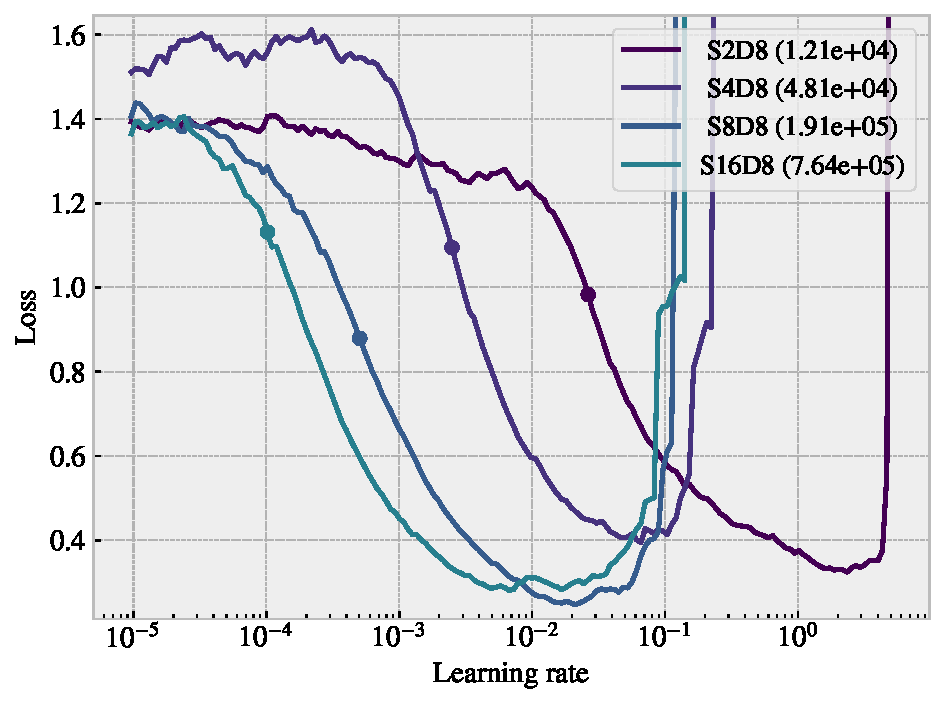
\includegraphics[width=\textwidth]{figures/ML/LR_range_specific.pdf}
      \caption{}
      % \label{fig:}
  \end{subfigure}
  \hfill
  \begin{subfigure}[t]{0.49\textwidth}
      \centering
      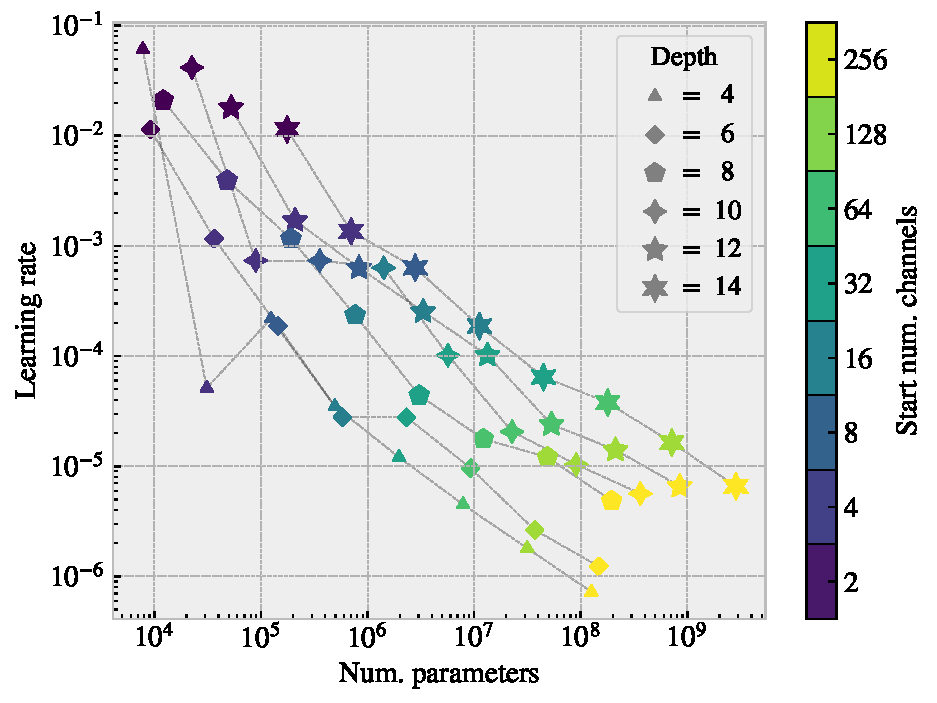
\includegraphics[width=\textwidth]{figures/ML/LR_range_full.pdf}
      \caption{}
      % \label{fig:}
  \end{subfigure}
  \hfill
  \caption{Learning rate range test for various model complexities. We increase the learning rate exponentially from num{e-7} to 10 during one epoch corresponding to an exponent increment of roughly $1/30$ per batch iteration. $(a)$ shows a few examples of the training loss history as a function of learning rate. The examplatory architectures are S[2, 16]D8 with the corresponding number of model parameters shown in parentheses in the legend. The dot indicates the suggested learning rate at the steepest decline of the slope. $(b)$ shows the full results of suggested learning rates depending on the number of model parameters with color coding differentiating the number of start channels and marker types differentiating different model depths. }
  \label{fig:LR_range}
\end{figure}
With the use of the suggested learning rates from \cref{fig:LR_range} we perform
a grid search over the corresponding $S$ and $D$ parameters. We evaluate both
the validation loss and the mean friction $R_2$ score which is shown in
\cref{fig:A_search_perf} together with the best epoch and the number of model
parameters. Additionally, we evaluate the mean friction $R_2$ score for a
selected set of configurations. This set consist of the top 10 configurations
with respect to maximum friction drop for the Tetrahedron and Honeycomb pattern
resepctively. This is done as a way of evaluating the performance on the
non-linear stretch curve which showed to be the more difficult patterns to
learn. The selected evaluation is shown in \cref{fig:A_search_compare}. Note
that these patterns are already a part of the full datset and thus the data points
related to these patterns are most likely present in both the training and the validation data set. Hence we cannot regard this as a validation set and the performance must be considered in conjuntion with the actual validation performance in \cref{fig:A_search_perf}.

\begin{figure}[H]
  \centering
  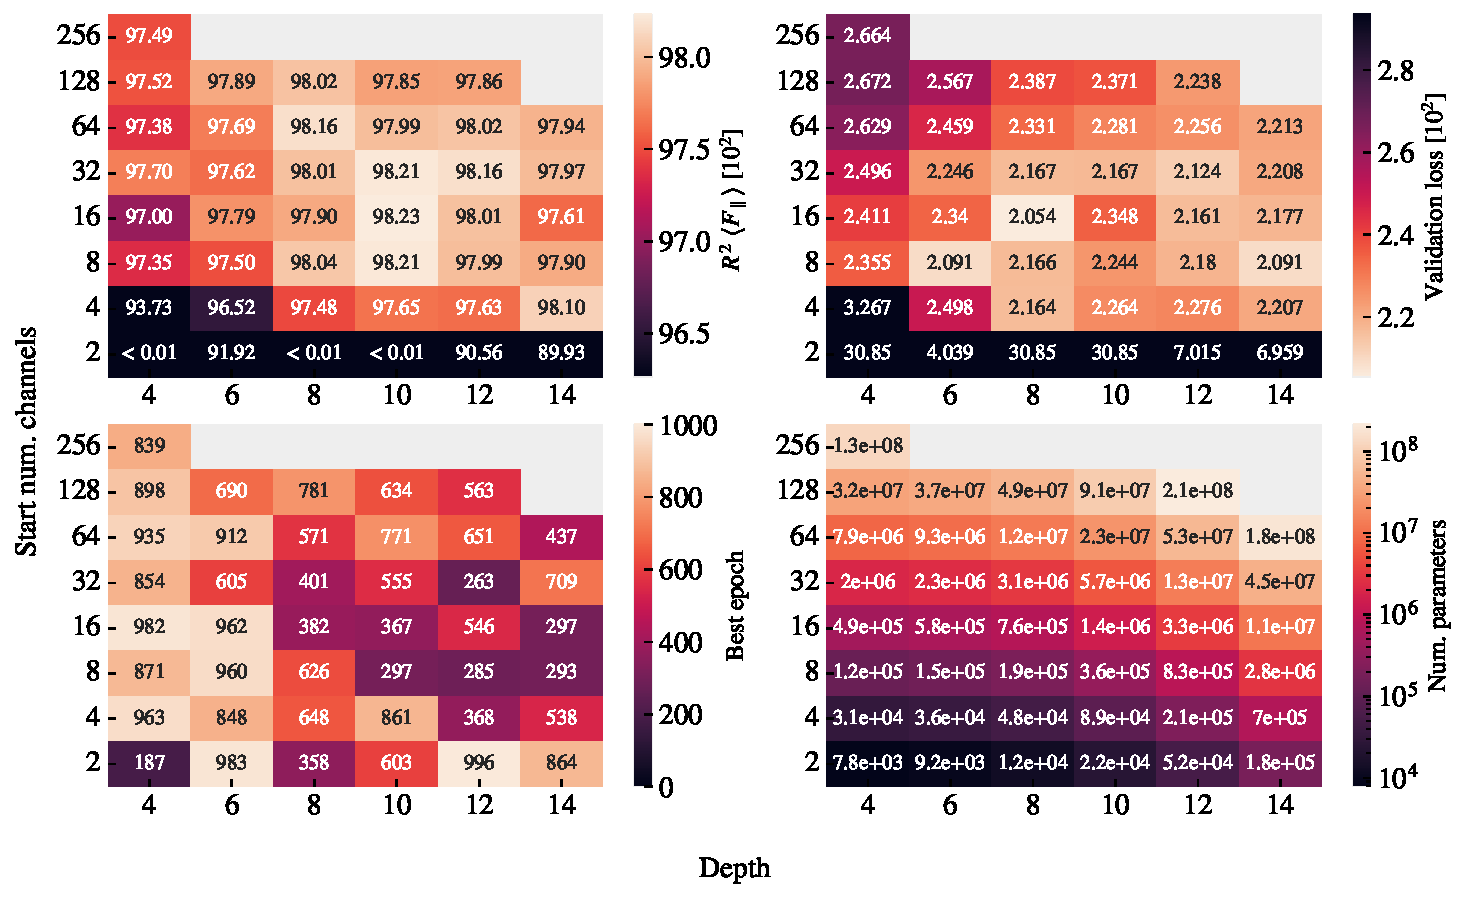
\includegraphics[width=\linewidth]{figures/ML/A_search_perf.pdf}
  \caption{Architecture search.}
  \label{fig:A_search_perf}
\end{figure}  

\begin{figure}[H]
  \centering
  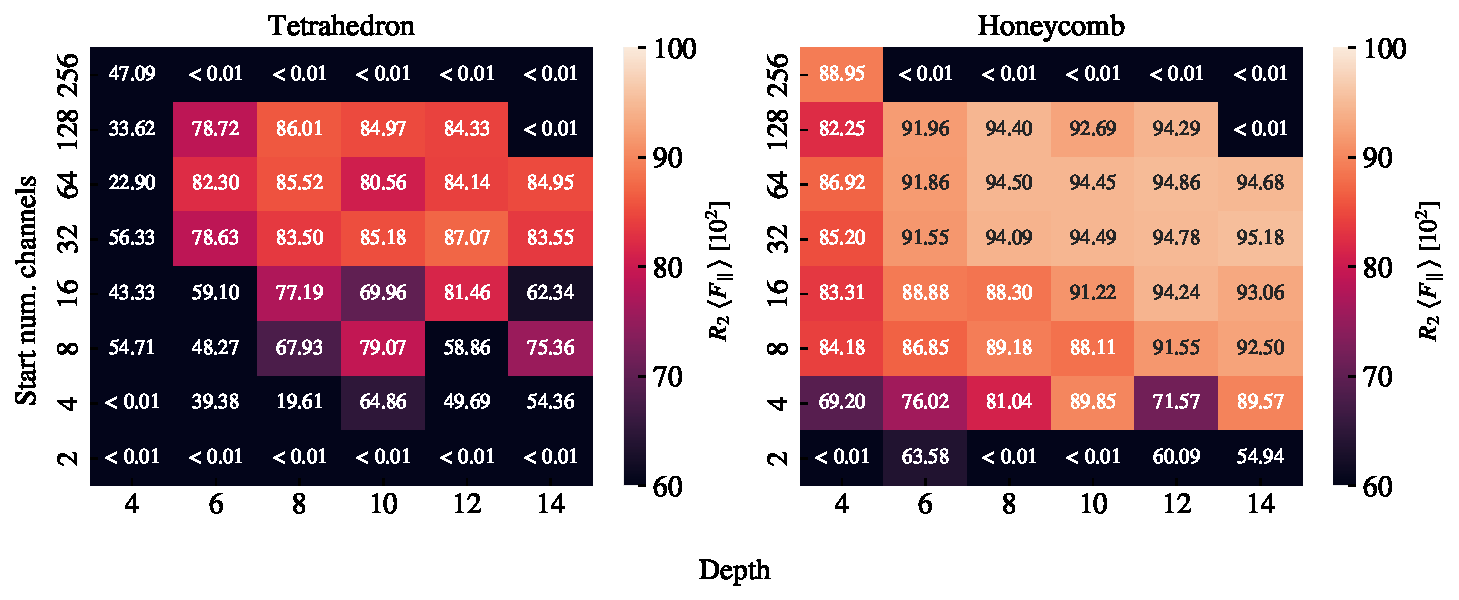
\includegraphics[width=\linewidth]{figures/ML/A_search_compare_perf}
  \caption{Selected pseudo validation set. \hl{Fix the missing grey fields in the top which are replaced by < 0.01.}}
  \label{fig:A_search_compare}
\end{figure}  

From the validation scores in \cref{fig:A_search_perf} we find that models
S(8-32)D(8-12) gives reasonble performance. When looking at the best epoch we
find that  models of low depth result in a later best epoch which is compatible
with underfitting. As the depth is increased we find more models with a lower
best epoch, in the range $\sim [300, 600]$, which on the other hand suggest
cases of overfitting. Since our training stores the best model during training,
we do not have to worry too much about overfitting, but we can take this
transistion from underfitting to overfitting as a sign that out search is
conducted in an appropiate complexity range. When consulting evaluation on the
selected set in \cref{fig:A_search_compare} we notice in general that we get
lower $R_2$ scores, especially for the Tetrahedron pattern, which shows that these constitute a challenge for the network. Considering that some of these datapoints is also present in the training data makes it even more clear that the network is not capturing the complexity in the data here. While the peak $R_2$ value for the validation score was found for the S16D10 model we see slightly preference for more complexity in the model with regard to the selected test. In the Tetrahedron grid search we find the best model to be S32D12, with a $R_2$ score of $\sim 87 \%$. This model choice is more or less compatible with the overall performance as this is among the top candidates for the for $R_2$ and loss in \cref{fig:A_search_perf} and the $R_2$ score for the Honeycomb pattern in \cref{fig:A_search_compare} as well. Hence, we settle on this model moving on to the setting of the momentum and weight decay parameter. 

We consider momentum $m$ and weight decays $wd$ in the range $m \in [0.85,
0.99]$ and $wd \in [0, 1e-2]$. An increased momentum is expected to decrease the
appropiate learning rate, and thus we perform a new learning rate range
test to determine a suitable choice for the learning rate for each momentum choice. We propose two learning rate schemes: A constant learning rate as used until this point and a one cycle policy. In the one cycle policy we set a maximum bound for the learning rate and start from a factor $1/20$ of this bound and increase towards the maximum bound during the first 30\% of the
training. We then decreases towards a final minimum being a factor $1e-4$ of the maximum bound during the remaining 70\% of training. The increase and decrease is done by a cosine function. The suggested learning rate for the constant learning rate scheme is once again determined by the steepest slope on the loss curve while the maximum bound used for the one cycle policy is determined as the point of diverging. We find that the minimum point on the loss curve is as suitable choice that approaches the diverging point without getting to close and causing
diverging learing. The learning rate range test for momentum is shown in \cref{fig:LR_range_mom}. Using the results for the momentum learning rate range test we perform a grid search of momentum and weight decay. We examine again the validation loss and validation mean friction $R_2$ score in addition to the friciton mean $R_2$ score for the selected set of Tetrahedron and Honeycomb patterns. This is shown for the constant learning rate scheme in \cref{fig:mom_weight_search_constant} and for the cyclic scheme in \cref{fig:mom_weight_search_cyclic}.

\begin{figure}[H]
  \centering
  \begin{subfigure}[t]{0.49\textwidth}
      \centering
      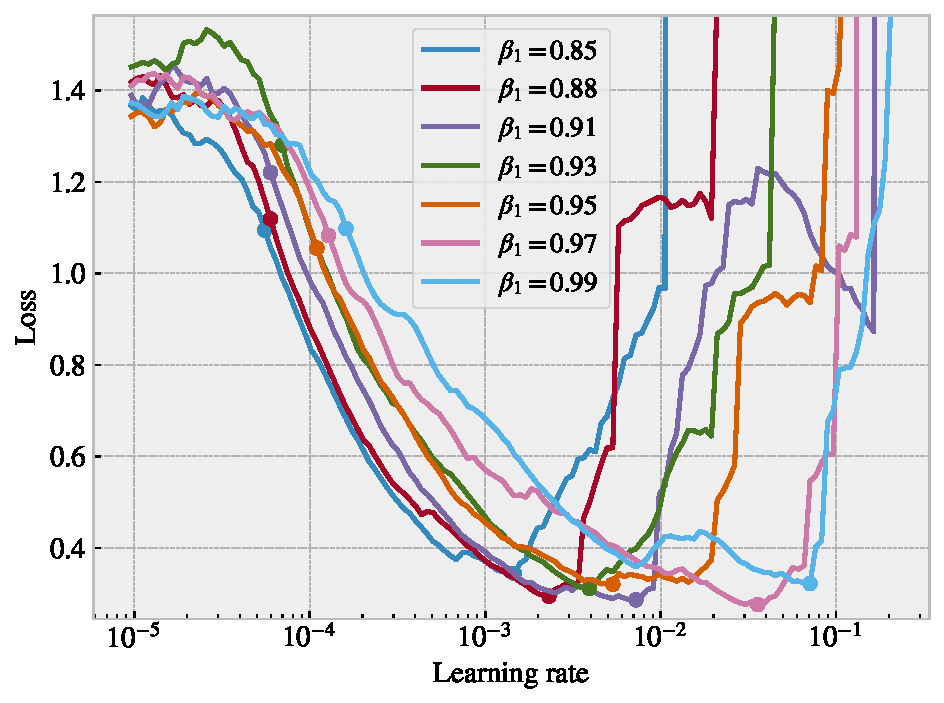
\includegraphics[width=\textwidth]{figures/ML/LR_momentum_test_a.pdf}
      \caption{}
      % \label{fig:}
  \end{subfigure}
  \hfill
  \begin{subfigure}[t]{0.49\textwidth}
      \centering
      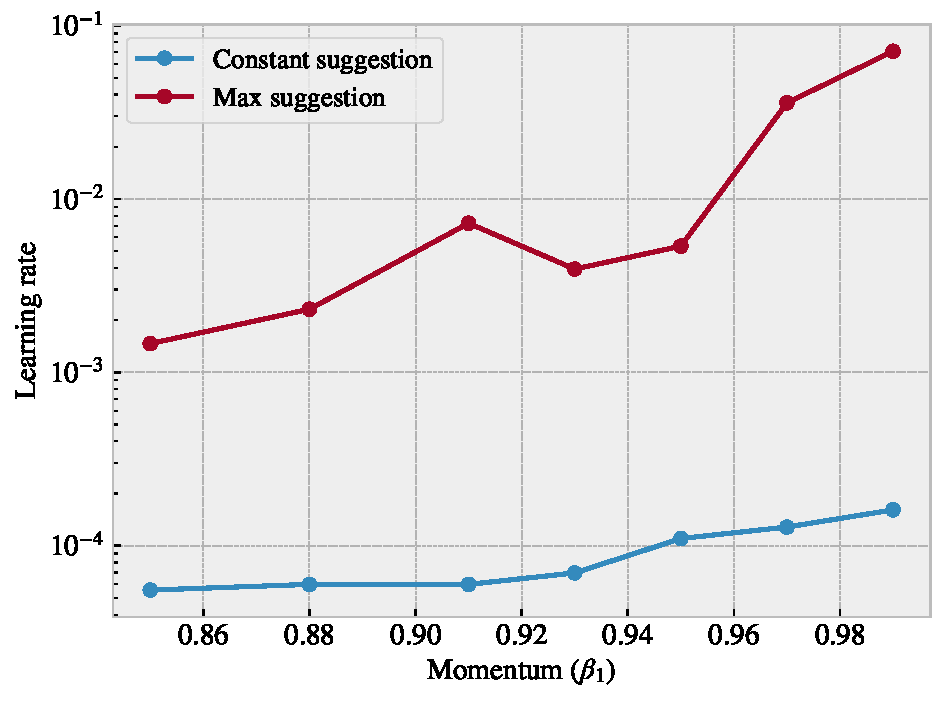
\includegraphics[width=\textwidth]{figures/ML/LR_momentum_test_b.pdf}
      \caption{}
      % \label{fig:}
  \end{subfigure}
  \hfill
  \caption{Momentum learning rate range tets}
  \label{fig:LR_range_mom}
\end{figure}


\begin{figure}[H]
  \centering
  \begin{subfigure}[t]{1.0\textwidth}
      \centering
      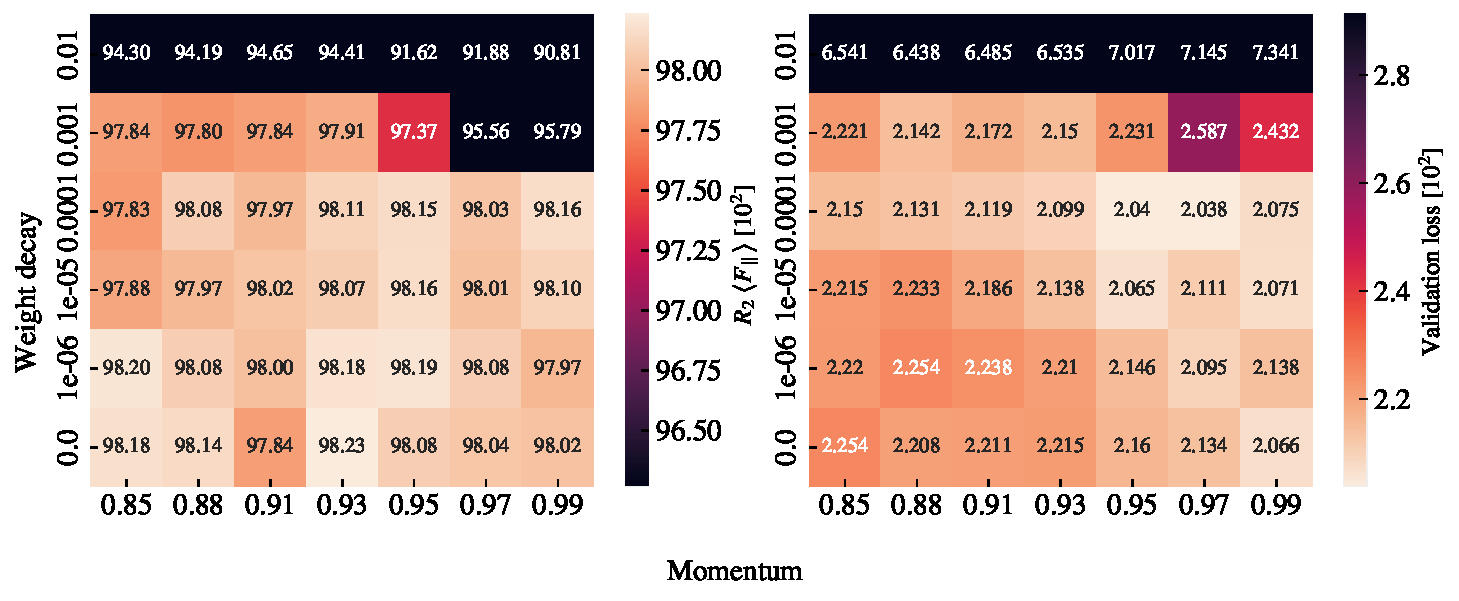
\includegraphics[width=\textwidth]{figures/ML/mom_weight_search_constant_perf.pdf}
      \caption{Performance}
      % \label{fig:}
  \end{subfigure}
  \hfill
  \begin{subfigure}[t]{1.0\textwidth}
      \centering
      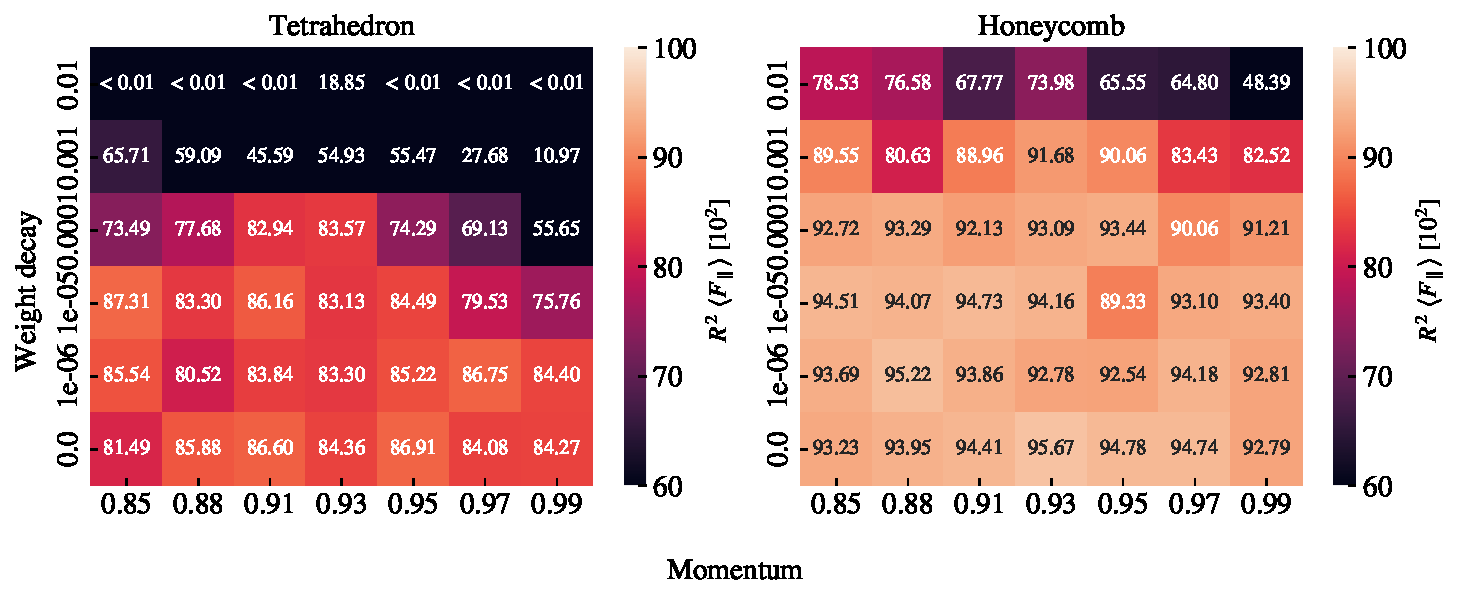
\includegraphics[width=\textwidth]{figures/ML/mom_weight_search_compare_constant_perf.pdf}
      \caption{Compare}
      % \label{fig:}
  \end{subfigure}
  \hfill
  \caption{Constant learing rate and momentum scheme}
  \label{fig:mom_weight_search_constant}
\end{figure}

\begin{figure}[H]
  \centering
  \begin{subfigure}[t]{1.0\textwidth}
      \centering
      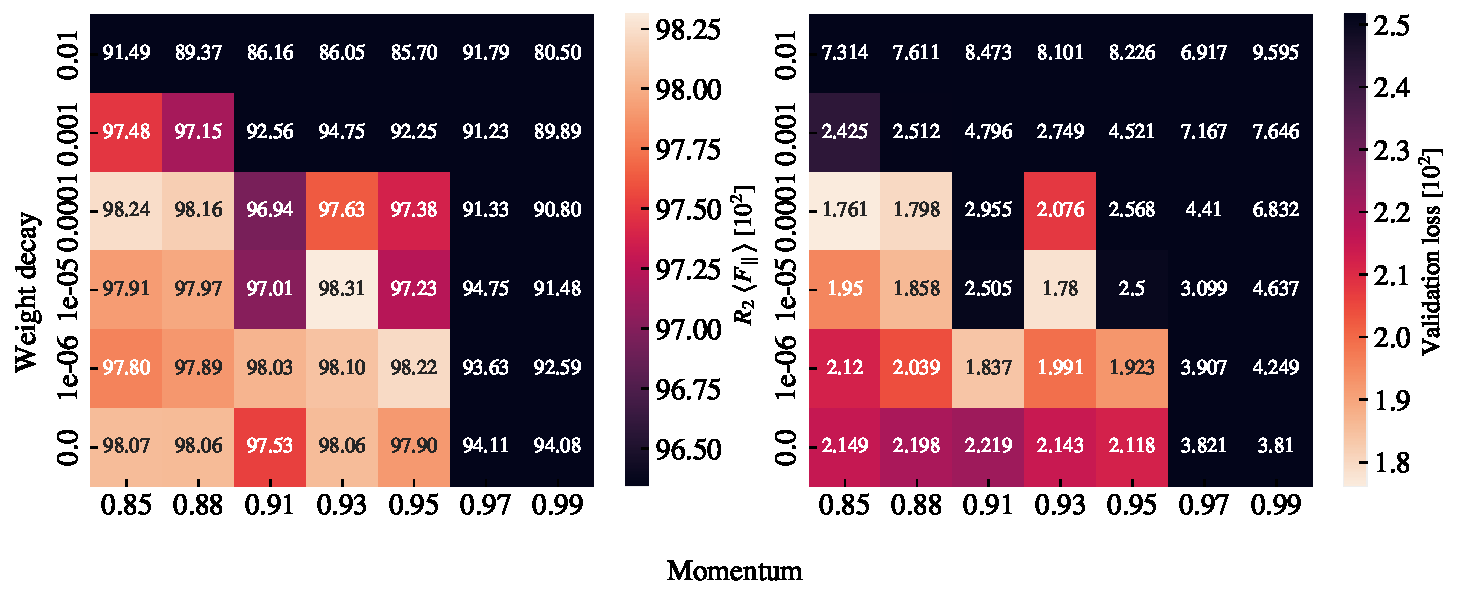
\includegraphics[width=\textwidth]{figures/ML/mom_weight_search_cyclic_perf.pdf}
      \caption{Performance}
      % \label{fig:}
  \end{subfigure}
  \hfill
  \begin{subfigure}[t]{1.0\textwidth}
      \centering
      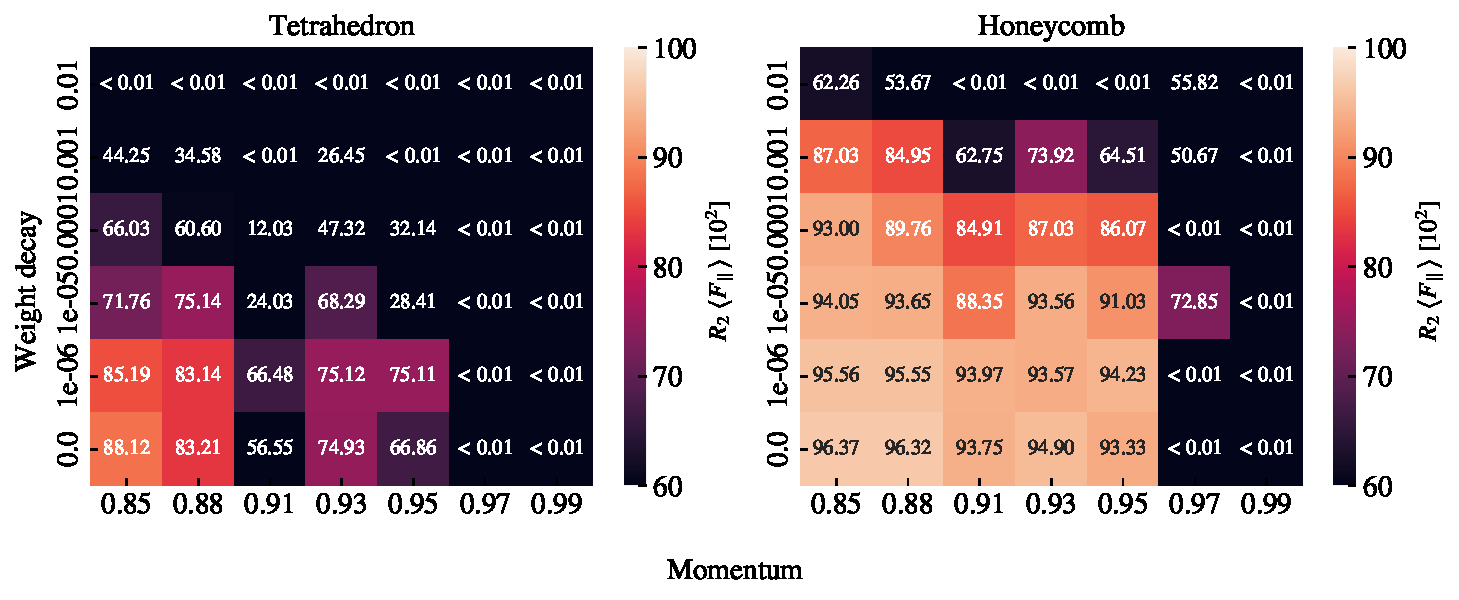
\includegraphics[width=\textwidth]{figures/ML/mom_weight_search_compare_cyclic_perf.pdf}
      \caption{Compare}
      % \label{fig:}
  \end{subfigure}
  \hfill
  \caption{Cyclic learing rate and momentum scheme}
  \label{fig:mom_weight_search_cyclic}
\end{figure}




The original validation scores, before varying momentum and weight decay, were a validation loss of 0.02124 and a mean friction $R_2$ score of 0.9816. By varying momentum and weight decay we are able to improve the performance metrics slightly for the constant learning rate scheme (loss: 0.02038, $R_2$: 0.9823) and even more for the cyclic scheme (loss: 0.0176, $R_2$: 0.9831), however notice that these scores a taking for their individual optimial hypersettings. The comparison among best scores are summarized in \cref{tab:mom_weight_search}. In general the
constant scheme shows reasonble stable results for all momentum settings $m \in
[0.85, 0.99]$ in combination with a low weight decay $wd \le \num{e-4}$. For the cyclic scheme the performance peaks towards a low momentum $m \le 0.93$ and low weight decay $wd \le \num{e-4}$. Looking at the summary in \cref{tab:mom_weight_search} we see that the cyclic scheme is able to produce a high score among all four performance metrics, however since these do not share common hyperparameters we need to make a choice here. 

\begin{table}[H]
  \begin{center}
  \caption{Momentum and weight decay grid search using S32D12 model.}
  \label{tab:mom_weight_search}
  \begin{tabular}{|c|c|c|c|c|} \hline
     &  & Score [\num{e2}] & Momentum & Weight decay \\ \hline
     \multirow{3}{*}{Validation loss} & Original & 2.124 & 0.9 & 0  \\ 
      & Constant & 2.038 & 0.97 & \num{e-4} \\ 
      & Cyclic & 1.761 & 0.85 & \num{e-4} \\ \hline
     \multirow{3}{*}{Validation $R_2$} & Original & 98.16 & 0.9 & 0  \\ 
      & Constant & 98.23 & 0.93 & 0 \\ 
      & Cyclic & 98.31 & 0.93 & \num{e-5} \\ \hline
     \multirow{3}{*}{Tetrahedron $R_2$} & Original & 87.07 & 0.9 & 0  \\ 
      & Constant & 87.31 & 0.85 & \num{e-5} \\ 
      & Cyclic & 88.12 & 0.85 & 0 \\ \hline
     \multirow{3}{*}{Honeycomb $R_2$} & Original & 94.78 & 0.9 & 0  \\ 
      & Constant & 95.67 & 0.93 & 0 \\ 
      & Cyclic & 96.37 & 0.85 & 0 \\ \hline
  \end{tabular}
  \end{center}
\end{table}

Look at overfitting via training history. 


% The LR range is done is arround 200 steps (before it diverges). So if I figure
% out the number of batches I can check how many epochs is default since number of
% steps is steps per epoch times number of epochs. 

% Seems like there are 242 batches in the full dataset so it probably just do one
% epoch...

% Argument for choosingt by selected set: Why rather want the model to be used to find a single configuration which is extrodinary than 10 descent designs. Thus we do not worry too much about safety

\subsection{Final model}

From the hypertuning study we choose the S32D12 model trained by a cylic training scheme with momentum 0.85 and weight decay 0. The main performance metrics are shown in \cref{tab:final_model_eval}. Since the porosity is a number between $0$ and $1$ we can interpret the absolute error as the percentage error similar to the relative error for the rupture stretch. The rupture stretch is generally within a 13 \% margin, but this number might especially high due to some low stretch rupture cases in the dataset. The stretch curves for mean friction, max friction and contact is shown in \cref{fig:final_model_eval} for the Tetrahedron (7, 5, 1) and Honeycomb (2,2,1,5) used in the pilot study. This gives a visual interpretation of how well the fits actually are for a given $R_2$ scores, and we notice that a $R_2$ score above 0.98 is certainly visually promising for capturing the non-linear in the data. 

\begin{table}[H]
  \begin{center}
  \caption{Mean values are used over different configurations.}
  \label{tab:final_model_eval}
  \begin{tabular}{ | c | c | c | c | c | c | c | c |} \hline
    & Loss [\num{e2}] & \multicolumn{3}{c|}{$R_2$ [\num{e2}]} & Abs. [\num{e2}] & Rel. [\num{e2}]  & Acc. [\num{e2}] \\ \hline
    & Total & Mean $F_f$ & Max $F_f$ & Contact & Porosity & Rup.\ Stretch & Rupture \\ \hline
  Validation  & 2.1488 & 98.067 & 93.558 & 94.598 & 02.325 & 12.958 & 96.102 \\ \hline
  Tetrahedron & 4.0328 & 88.662 & 85.836 & 64.683 & 01.207 & 05.880 & 99.762 \\ \hline
  Honeycomb   & 8.6867 & 96.627 & 89.696 & 97.171 & 01.040 & 01.483 & 99.111 \\ \hline
  \end{tabular}
  \end{center}
\end{table}


\begin{figure}[H]
  \centering
  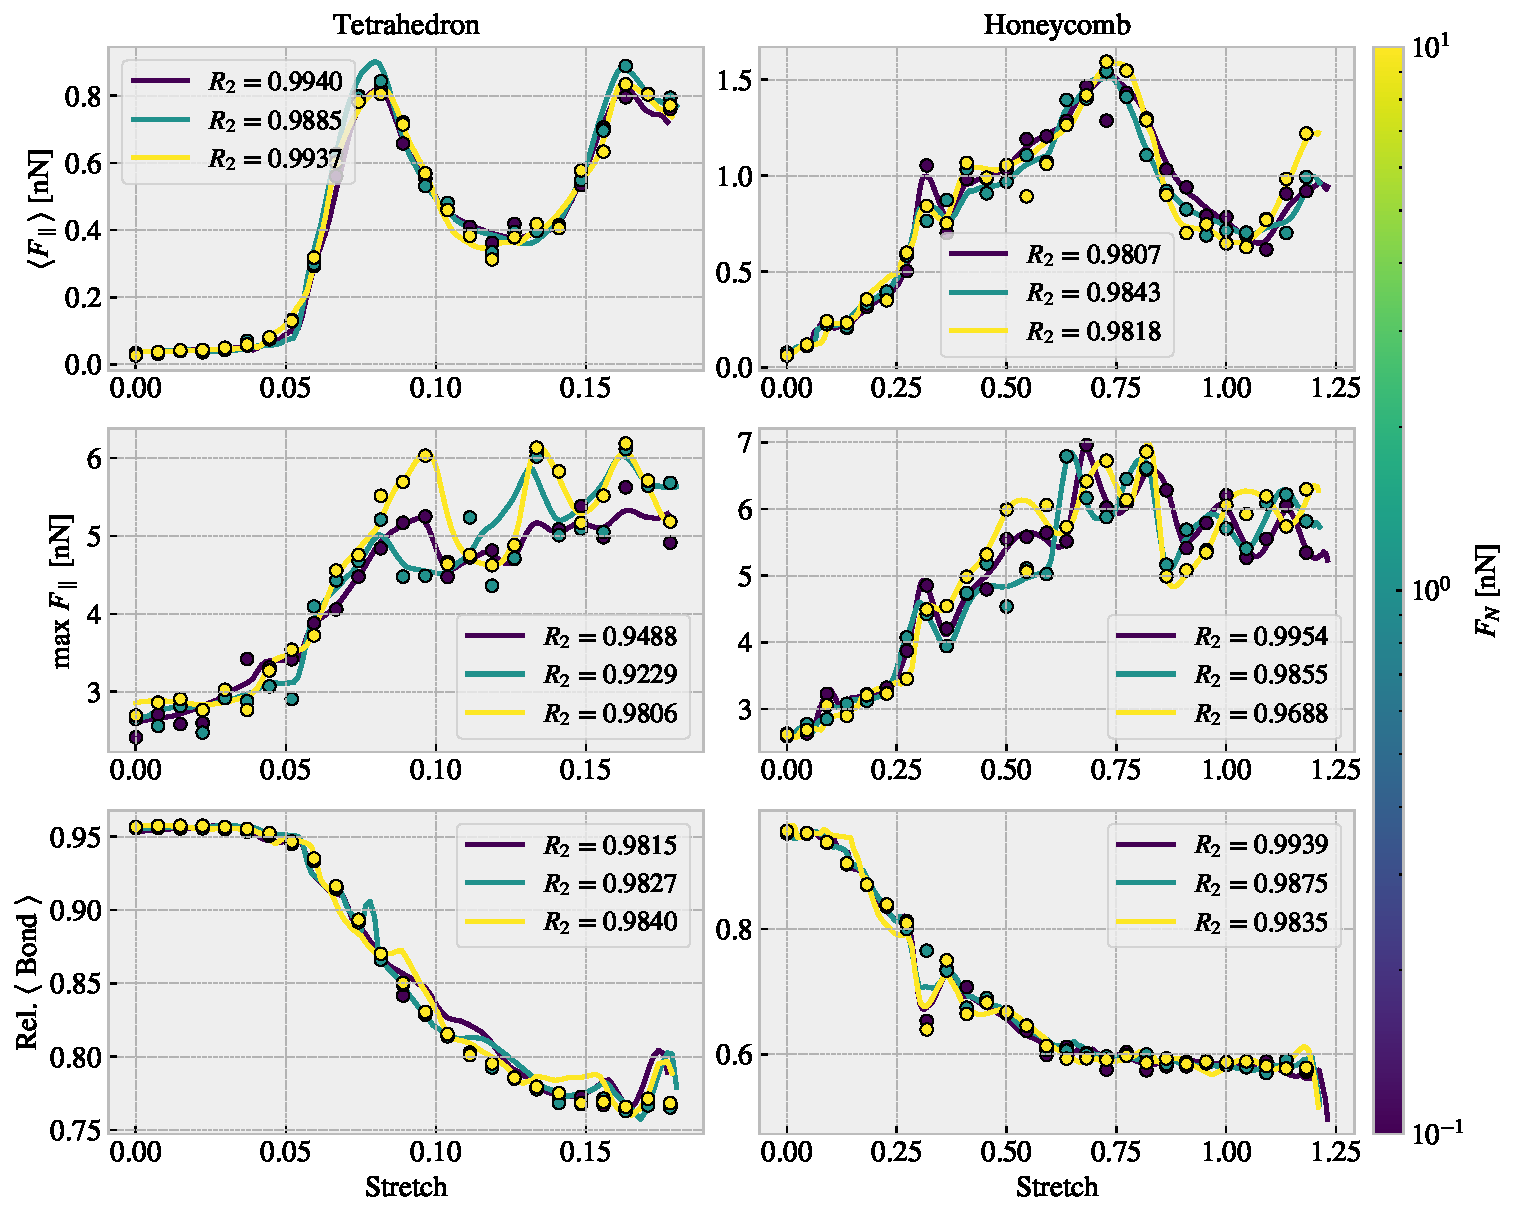
\includegraphics[width=\linewidth]{figures/ML/final_model_evaluation.pdf}
  \caption{With \num{e3} points in the stretch range [0, 1.5] and stopping after first rupture True prediction.}
  \label{fig:final_model_eval}
\end{figure}  

Having a trained model, we evaluate the performance for the top ranking within
the properties of interest. That is, we go through all the configurations in the
dataset for the Tetrahedron (\cref{tab:ML_ranking_pop}), Honeycomb
(\cref{tab:ML_ranking_hon}) and Random Walk (\cref{tab:ML_ranking_RW}) patterns
seperately and rank the configurations in each property category. This is then compared to the actual ranking in the dataset. Generally, we find that the \acrshort{ML} performs rather well in the ranking of the max, max difference and max drop property, but it is deviating a bit more for the minimum friction property. This is most likely due to the fact that the difference in minimum value is quite small compared to that in the max categories. The \acrshort{ML} model gives stable prediction for the max-categories for the Tetrahedron and Honeycomb pattern, but struggles a bit more for the Random Walk. Looking at the values for the top candidates in the max-types properties we see
that it is generally within a $\sim 0.2$ nN range which is promising. 

\begin{table}[H]
  \begin{center}
  \caption{Tetrahedon}
  \label{tab:ML_ranking_pop}
  \begin{tabular}{|c|c|c?{0.3mm}c|c|c|} \hline
    ML & \multicolumn{2}{c?{0.3mm}}{Data} &  \multicolumn{2}{c|}{\acrshort{ML}} & Data \\ \cline{2-5}
    Rank & Config & Value [nN] & Config & Value [nN] & Rank \\ \hline
    \multicolumn{6}{|c|}{Min $F_{\text{fric}}$} \\ \hline
    20 & (3, 9, 4) & 0.0067 & (3, 1, 2) & 0.0041 & 5  \\ \hline
    5 & (3, 1, 3) & 0.0075 & (1, 3, 4) & 0.0049 & 11 \\ \hline
    6 & (5, 3, 4) & 0.0084 & (1, 3, 3) & 0.0066 & 6  \\ \hline
    21 & (1, 7, 3) & 0.0084 & (3, 1, 4) & 0.0066 & 8  \\ \hline
    1 & (3, 1, 2) & 0.0097 & (3, 1, 3) & 0.0078 & 2  \\ \hline
    \multicolumn{6}{|c|}{Max $F_{\text{fric}}$} \\ \hline
    1 & (5, 3, 1) & 1.5875 & (5, 3, 1) & 1.5920 & 1 \\ \hline
    2 & (1, 3, 1) & 1.4310 & (1, 3, 1) & 1.2739 & 2 \\ \hline
    4 & (3, 1, 2) & 1.0988 & (9, 3, 1) & 1.1162 & 4 \\ \hline
    3 & (9, 3, 1) & 1.0936 & (3, 1, 2) & 0.7819 & 3 \\ \hline
    5 & (7, 5, 1) & 0.7916 & (7, 5, 1) & 0.7740 & 5 \\ \hline
    \multicolumn{6}{|c|}{Max $\Delta F_{\text{fric}}$} \\ \hline
    1 & (5, 3, 1) & 1.5529 & (5, 3, 1) & 1.5578 & 1 \\ \hline 
    2 & (1, 3, 1) & 1.3916 & (1, 3, 1) & 1.2331 & 2 \\ \hline 
    4 & (3, 1, 2) & 1.0891 & (9, 3, 1) & 1.0807 & 4 \\ \hline 
    3 & (9, 3, 1) & 1.0606 & (3, 1, 2) & 0.7778 & 3 \\ \hline 
    5 & (7, 5, 1) & 0.7536 & (7, 5, 1) & 0.7399 & 5 \\ \hline 
    \multicolumn{6}{|c|}{Max drop} \\ \hline
    1 & (5, 3, 1) & 0.8841 & (5, 3, 1) & 0.8603 & 1 \\ \hline 
    2 & (3, 5, 1) & 0.4091 & (3, 5, 1) & 0.3722 & 2 \\ \hline 
    4 & (7, 5, 1) & 0.3775 & (1, 1, 1) & 0.2879 & 5 \\ \hline 
    5 & (9, 7, 1) & 0.2238 & (7, 5, 1) & 0.2478 & 3 \\ \hline 
    3 & (1, 1, 1) & 0.1347 & (9, 7, 1) & 0.1302 & 4 \\ \hline 
  \end{tabular}
  \end{center}
\end{table}

\begin{table}[H]
  \begin{center}
  \caption{Honeycomb}
  \label{tab:ML_ranking_hon}
  \begin{tabular}{|c|c|c?{0.3mm}c|c|c|} \hline
    ML & \multicolumn{2}{c?{0.3mm}}{Data} &  \multicolumn{2}{c|}{\acrshort{ML}} & Data \\ \cline{2-5}
    Rank & Config & Value [nN] & Config & Value [nN] & Rank \\ \hline
    \multicolumn{6}{|c|}{Min $F_{\text{fric}}$} \\ \hline
    1 & (2, 5, 1, 1) & 0.0177 & (2, 5, 1, 1) & 0.0113 & 1 \\ \hline 
    9 & (2, 4, 5, 1) & 0.0187 & (2, 5, 5, 3) & 0.0149 & 7 \\ \hline 
    7 & (2, 4, 1, 1) & 0.0212 & (2, 5, 5, 1) & 0.0182 & 4 \\ \hline 
    3 & (2, 5, 5, 1) & 0.0212 & (2, 5, 3, 1) & 0.0186 & 5 \\ \hline 
    4 & (2, 5, 3, 1) & 0.0226 & (2, 4, 1, 3) & 0.0198  & 15 \\ \hline 
    \multicolumn{6}{|c|}{Max $F_{\text{fric}}$} \\ \hline
    1 & (2, 1, 1, 1) & 2.8903 & (2, 1, 1, 1) & 2.9171 & 1 \\ \hline 
    2 & (2, 1, 5, 3) & 2.2824 & (2, 1, 5, 3) & 2.4004 & 2 \\ \hline 
    6 & (2, 1, 3, 1) & 2.0818 & (2, 1, 5, 1) & 2.1060 & 5 \\ \hline 
    4 & (2, 1, 3, 3) & 2.0313 & (2, 1, 3, 3) & 1.9458 & 4 \\ \hline 
    3 & (2, 1, 5, 1) & 2.0164 & (2, 4, 1, 1) & 1.9381 & 6 \\ \hline 
    \multicolumn{6}{|c|}{Max $\Delta F_{\text{fric}}$} \\ \hline
    1 & (2, 1, 5, 3) & 2.0234 & (2, 1, 5, 3) & 2.1675 & 1 \\ \hline 
    2 & (2, 1, 1, 1) & 1.9528 & (2, 1, 1, 1) & 2.0809 & 2 \\ \hline 
    3 & (2, 4, 1, 1) & 1.8184 & (2, 4, 1, 1) & 1.9157 & 3 \\ \hline 
    4 & (2, 1, 3, 3) & 1.7645 & (2, 1, 3, 3) & 1.6968 & 4 \\ \hline 
    5 & (2, 4, 1, 3) & 1.4614 & (2, 4, 1, 3) & 1.5612 & 5 \\ \hline 
    \multicolumn{6}{|c|}{Max drop} \\ \hline
    1 & (2, 3, 3, 3) & 1.2785 & (2, 3, 3, 3) & 1.3642 & 1 \\ \hline 
    2 & (2, 1, 3, 1) & 1.1046 & (2, 1, 3, 1) & 0.9837 & 2 \\ \hline 
    3 & (2, 3, 3, 5) & 0.8947 & (2, 3, 3, 5) & 0.9803 & 3 \\ \hline 
    4 & (2, 1, 5, 3) & 0.8638 & (2, 1, 5, 3) & 0.9556 & 4 \\ \hline 
    13 & (2, 5, 1, 1) & 0.8468 & (2, 4, 5, 3) & 0.8999 & 8 \\ \hline 
  \end{tabular}
  \end{center}
\end{table}


\begin{table}[H]
  \begin{center}
  \caption{RW}
  \label{tab:ML_ranking_RW}
  \begin{tabular}{|c|c|c?{0.3mm}c|c|c|} \hline
    ML & \multicolumn{2}{c?{0.3mm}}{Data} &  \multicolumn{2}{c|}{\acrshort{ML}} & Data \\ \cline{2-5}
    Rank & Config & Value [nN] & Config & Value [nN] & Rank \\ \hline
    \multicolumn{6}{|c|}{Min $F_{\text{fric}}$} \\ \hline
    1 & 12 & 0.0024 & 12 & -0.0011 & 1 \\ \hline 
    24 & 76 & 0.0040 & 06 & 0.0036  & 27 \\ \hline 
    6 & 13 & 0.0055 & 14 & 0.0074  & 23 \\ \hline 
    31 & 08 & 0.0065 & 05 & 0.0082  & 19 \\ \hline 
    26 & 07 & 0.0069 & 63 & 0.0085  & ? \\ \hline 
    \multicolumn{6}{|c|}{Max $F_{\text{fric}}$} \\ \hline
    3 & 96 & 0.5758 & 99 & 0.5155 & 2 \\ \hline 
    1 & 99 & 0.5316 & 98 & 0.4708 & 3 \\ \hline 
    2 & 98 & 0.4478 & 96 & 0.4356 & 1 \\ \hline 
    4 & 97 & 0.3624 & 97 & 0.3503 & 4 \\ \hline 
    11 & 58 & 0.3410 & 55 & 0.2817 & 7 \\ \hline 
    \multicolumn{6}{|c|}{Max $\Delta F_{\text{fric}}$} \\ \hline
    3 & 96 & 0.5448 & 99 & 0.4669 & 2 \\ \hline 
    1 & 99 & 0.4769 & 98 & 0.4314 & 3 \\ \hline 
    2 & 98 & 0.4085 & 96 & 0.4128 & 1 \\ \hline 
    4 & 97 & 0.3268 & 97 & 0.3080 & 4 \\ \hline 
    78 & 57 & 0.2978 & 55 & 0.2542 & 7 \\ \hline 
    \multicolumn{6}{|c|}{Max drop} \\ \hline
    3 & 01 & 0.1818 & 00 & 0.1883 & 3 \\ \hline 
    2 & 96 & 0.1733 & 96 & 0.1654 & 2 \\ \hline 
    1 & 00 & 0.1590 & 01 & 0.1532 & 1 \\ \hline 
    11 & 37 & 0.1022 & 04 & 0.0591 & 8 \\ \hline 
    28 & 34 & 0.0879 & 56 & 0.0552 & 20 \\ \hline 
  \end{tabular}
  \end{center}
\end{table}




\section{Accelerated Search}

We use the \acrshort{ML} model perform a search through new configurations which optimize our properties of interest. We approach this search by two different methods:
\begin{enumerate}
  \item Using the generative algorithms developed for the creation of the Tetrahedron, Honeycomb and Random walk patterns, we create an extended dataset and evaluate the performance using the \acrshort{ML}.
  \item Using the genetic algoritm method we pertubate the configurations and optimize for the maximum drop property using the \acrshort{ML} model to evaluate the fitness function. 
\end{enumerate}


\subsection{Patteren generation search}
% Judging from the ranking in \cref{tab:ML_ranking_pop}, \cref{tab:ML_ranking_hon} and
% \cref{tab:ML_ranking_RW}, the \acrshort{ML} model showcases a reasonable
% performance with respect to the task of assigning ordinal numbers, i.e.\ predictiong the relative ranking, to the configurations. 

We utilize the pattern generators to create an extended dataset for our search. For the Tetrahedron and Honeycomb patterns, the increment of the parameters will eventually lead to the main structures becoming so large they do not really fit on the sheet anymore. Thus, we can essentially perform a
full search ``maxing out'' the parameters of these patterns. We estimate
that this is done with the max parameters, $(60, 60, 30)$ for the Tetrahedron,
and $([30, 30, 30, 60])$ for the Honeycomb. We use a random reference position
and regenerate each unique parameter 10 times to explore translational effects. This gives in total 135k configurations for the
Tetrahedron pattern and 2025k for the Honeycomb pattern. For the Random walk
generator, we do a Monte Carlo sampling. In each sample we draw the scalar values, either from an uniform (U) or logarithmic uniform (LU) distribution as follows.
\begin{align*}
  \text{Num. walks} &\sim \text{U}[1, 30] & \text{Max. steps} &\sim \text{U}[1,30]  & \text{Min. dis.} &\sim \text{U}[0,4] \\
  \text{Bias direction} &\sim \text{U}[0, 2\pi] & \text{Bias. strength} &\sim \text{LU}[0,10]  & p_{\text{stay}} &\sim \text{U}[0,1]  
\end{align*}
Notice that we use discrete distribution for the parameters requiring integers. For the binary parameters \textit{Connection}, \textit{Avoid unvalid},
\textit{RN6} and \textit{Grid start} we simply set the values by 50--50 chance. The
remaining parameters are kept constant at \textit{Periodic: True} and \textit{Centering:
False} throughout the search. For the handling of clustering we implement the
repair algorithm such that the sheet is repaired by the least modifications
approach rather than retrying several times \hl{Make sure that this is
introduced somewhere}. Due to the extra computation time associated with the
random walk and the repair algorithm, we only generate 10k configurations within
this class. For the evaluation of the configurations we use a normal load of \SI{5}{nN} and generate a stretch curve in the domain 0--200 \% using 100 evenly spacd points. top candidate results for each property are shown in
\cref{tab:pattern_search} including a comparison to the dataset top candidates
originally shown in \cref{tab:data_properties}. The random walk top five candidates are visualized in \cref{fig:RW_search_top5}.

First of all, the search gives a rather consistent result regarding the minimization of friction where the top candidates all share the same feature of being sparsely cut. For the Random Walk we see this clearly in\cref{fig:RW_search_top5}, while for the Tetrahedon and Honeycomb patterns this is evident from the configuration parameters shown in
\cref{tab:pattern_search} where the parameters reveal a high spacing between the
cuts. The porosity of the minimum friction top candidates are $1.5\%, 5.6\%, 1.6\%$ for the
Tetrahedron, Honeycomb and Random walk respectively. These results point towards the fact that the kirigami modification does not immediately give rise to any lowering of friction (within our \acrshort{MD} parameter domain).

Note that the full ranking did not strictly favor the least amount of
atoms removed, but considering that the relative error is high for this domain we can not expect this kind of precision. The fact that the top candidates all take
negative values also shows that the model is not reliable in this domain. By
asking for the lowest friction we essentially find the weak spots, sparsely populated points in \hl{vector space},  which can lead to unphysical predictions. This problem should most likely be resolved through an extension of the dataset and perhaps by applying a physical constraint to the
model regarding negative values. 

Among the remaining properties, we find competing values for the Honeycomb and Random walk classes only. When taking a closer look to the ranking for each property it became apparent the predictions are highly sensitive
to the reference position parameters used for the Tetrahedron and Honeycomb
pattern. Since we repeated each parameter 10 times with random reference positions, we initially expected to get a ranking in sets of 10. However, the ranking only shows contiguous appearing sets in the range 1--5. Hence we investigate this sensitivity further by evaluating the scores for a systematic change of the reference position for selected configurations. We generally found the mac drop parameter to give the highest variation and thus we show scores for the max drop top candidates, Tetrahedron $(1,7,1)$, $(5,3,1)$ and Honeycomb $(3,3,5,3)$, $(2,3,3,3)$, in
\cref{fig:ref_search_top_data}. It becomes evident that the predictions vary
drastically with translation of these patterns. The emerging question is then whether this is actually grounded in a physical phenomenon or simply a deficiency in the \acrshort{ML}. Even though the patterns are periodic in the x-y-plane, by the number of center elements represented by the shown squares in \cref{fig:ref_search_top_data}, the translation will determine the specific configuration of the edge. Previous studies of static friction and stick-slip behavior point to the importance of edge effects \hl{look back at theory and
maybe source}, and thus for a sheet where the atoms sitting on the $\pm x$ free sides constitutes about 2.5\% of the inner sheet atom count, it is not unreasonable
that the translation might result in a significantly different outcome. In that case, the search through reference positions highlights that the translation can be key to optimizing for certain properties. However, the results might also indicate that the model is either overfitted or that we simply did not provide enough data to reach a generalization of the complex physical behavior of the system. The sensible way forward to unravel this would be to generate additional
translational variants of the same configurations to investigate for any physical edge dependencies or otherwise strengthen the model. We earmark this suggestion for another study. When considering some of the stretch curves we also find that the prediction of the rupture point makes a crucial impact. As the rupture was often predicted on a descending part of the curve any variation to the rupture point will affect the max drop property quite significantly.





\begin{table}[H]
  \begin{center}
  \caption{Pattern search. The values are in units nN.}
  \label{tab:pattern_search}
  \begin{tabular}{|L{1.75cm} |c|c|c| c |c|c|c|} \cline{2-4} \cline{6-8}
  \multicolumn{1}{c|}{} & \multicolumn{3}{c|}{Search}  && \multicolumn{3}{c|}{Data} \\ \cline{2-4} \cline{6-8}
  \multicolumn{1}{c|}{\textbf{Scores}} & Tetrahedron & Honeycomb & Random walk && Tetrahedron & Honeycomb & Random walk \\ \cline{1-4} \cline{6-8}
  Min $F_{\text{fric}}$         & $-0.062 \ \ $  & $-0.109 \ \ $  & $-0.061 \ \ $ &&   0.0067 & 0.0177 & 0.0024 \\ \cline{1-4} \cline{6-8}
  Max $F_{\text{fric}}$         & $1.089$        & $2.917$        & $0.660$       &&   1.5875 & 2.8903 & 0.5758 \\ \cline{1-4} \cline{6-8}
  Max $\Delta F_{\text{fric}}$  & $1.062$        & $2.081$        & $0.629$       &&   1.5529 & 2.0234 & 0.5448 \\ \cline{1-4} \cline{6-8}   
  Max drop                      & $0.277$        & $1.250$        & $0.269$       &&   0.8841 & 1.2785 & 0.1818 \\ \cline{1-4} \cline{6-8}   
  \multicolumn{8}{c|}{} \\ \cline{2-4} \cline{6-8}
  \multicolumn{1}{c|}{\textbf{Configs.}} & Tetrahedron & Honeycomb & Random walk  && Tetrahedron & Honeycomb & Random walk  \\ \cline{1-4} \cline{6-8}
  Min $F_{\text{fric}}$         & $(13,11,14)$ & $(14,25,7,19)$  & No naming &&   $(3,9,4)$ & $(2,5,1,1)$ & 12 \\ \cline{1-4} \cline{6-8}
  Max $F_{\text{fric}}$         & $(1,3,1)$    & $(2,1,1,1)$     & No naming &&   $(5,3,1)$ & $(2,1,1,1)$ & 96 \\ \cline{1-4} \cline{6-8}
  Max $\Delta F_{\text{fric}}$  & $(1,3,1)$    & $(2,1,1,1)$     & No naming &&   $(5,3,1)$ & $(2,1,5,3)$ & 96 \\ \cline{1-4} \cline{6-8}   
  Max drop                      & $(1,7,1)$    & $(3,3,5,3)$     & No naming &&   $(5,3,1)$ & $(2,3,3,3)$ & 01 \\ \cline{1-4} \cline{6-8}   
  \end{tabular}
  \end{center}
\end{table}


\begin{figure}[H]
  \centering
  \begin{subfigure}[t]{0.49\textwidth}
      \centering
      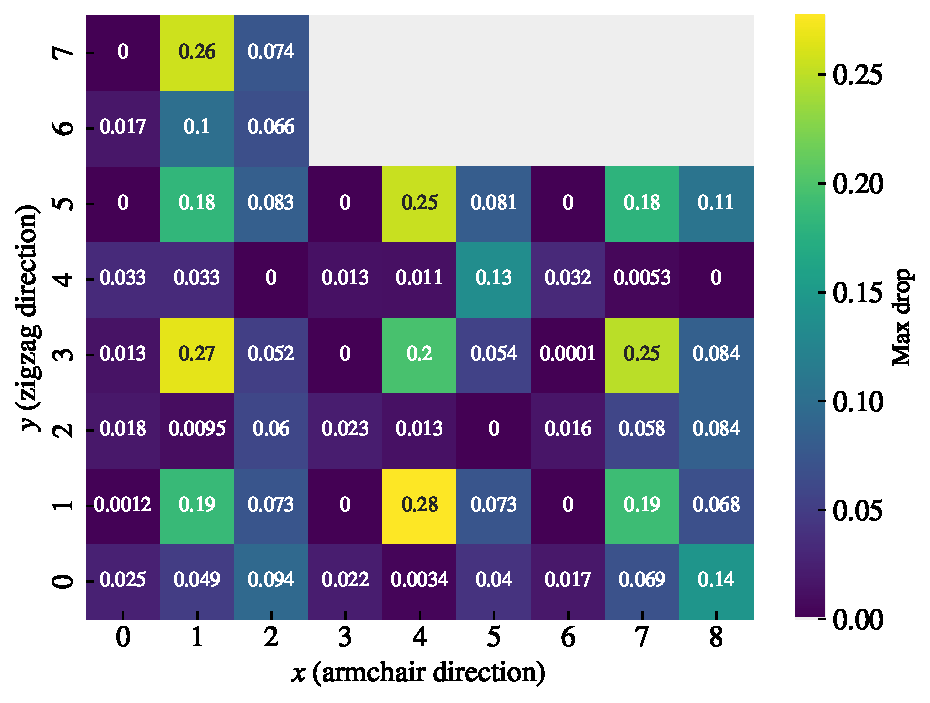
\includegraphics[width=\textwidth]{figures/search/ref_search_drop_pop_1_7_1_ref_search.pdf}
      \caption{Tetrahedron $(1,7,1)$ (60). Std = 0.08, Rel.\ Std = 1.13}
      % \label{fig:}
  \end{subfigure}
  \hfill
  \begin{subfigure}[t]{0.49\textwidth}
    \centering
    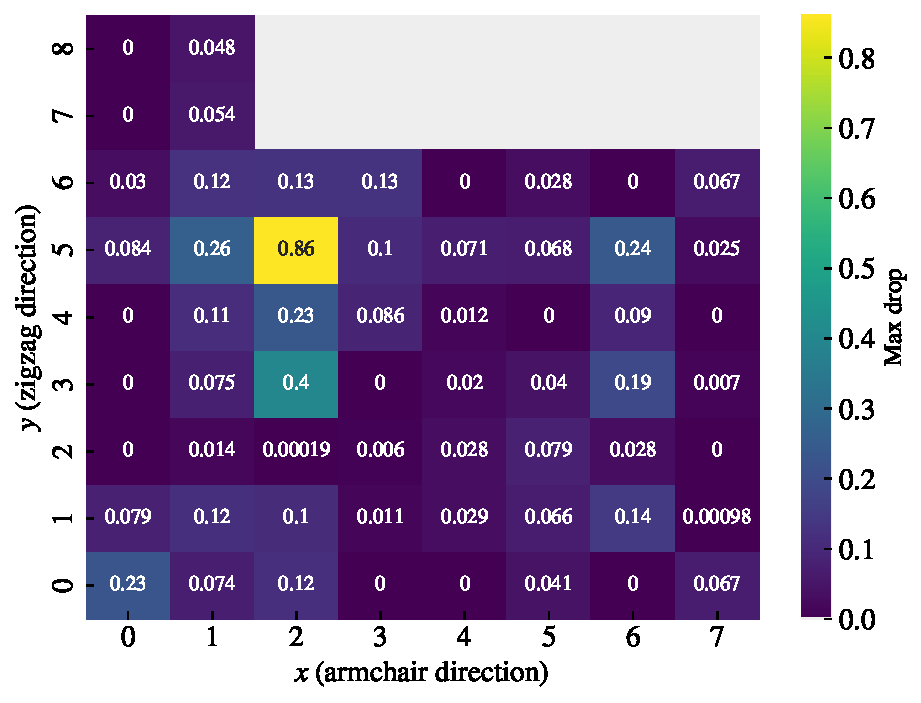
\includegraphics[width=\textwidth]{figures/search/ref_search_drop_pop_5_3_1_ref_search.pdf}
    \caption{Tetrahedron $(5,3,1)$ (60). Std = 0.13, Rel.\ Std = 1.61}
    % \label{fig:}
  \end{subfigure}
  \hfill
  \begin{subfigure}[t]{0.49\textwidth}
      \centering
      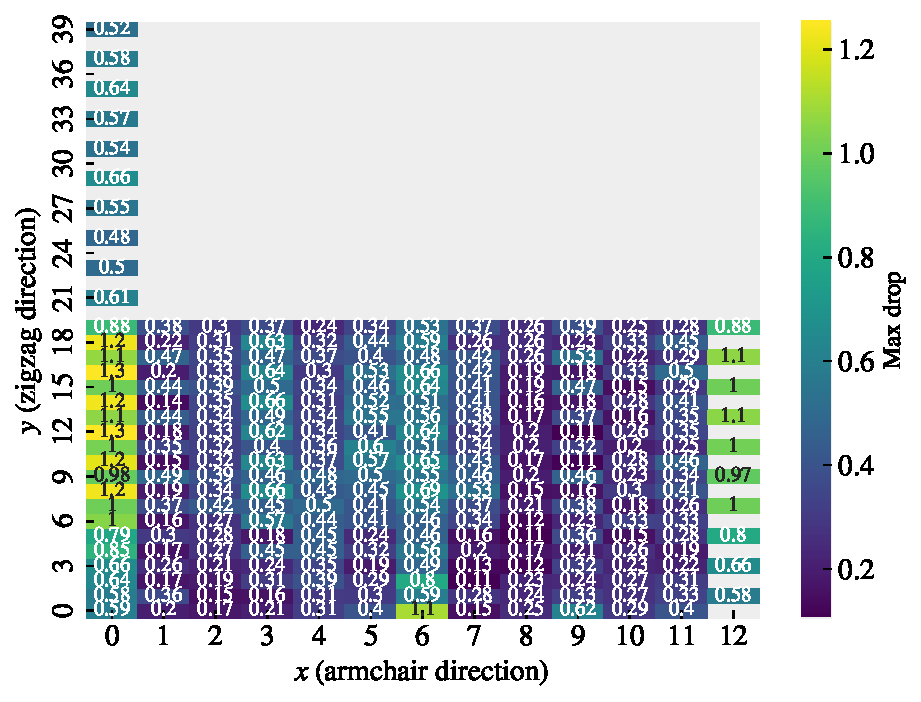
\includegraphics[width=\textwidth]{figures/search/ref_search_drop_hon_3_3_5_3_ref_search.pdf}
      \caption{Honeycomb $(3,3,5,3)$ (260). Std = 0.25, Rel.\ Std = 0.58}
      % \label{fig:}
  \end{subfigure}
  \hfill
  \begin{subfigure}[t]{0.49\textwidth}
      \centering
      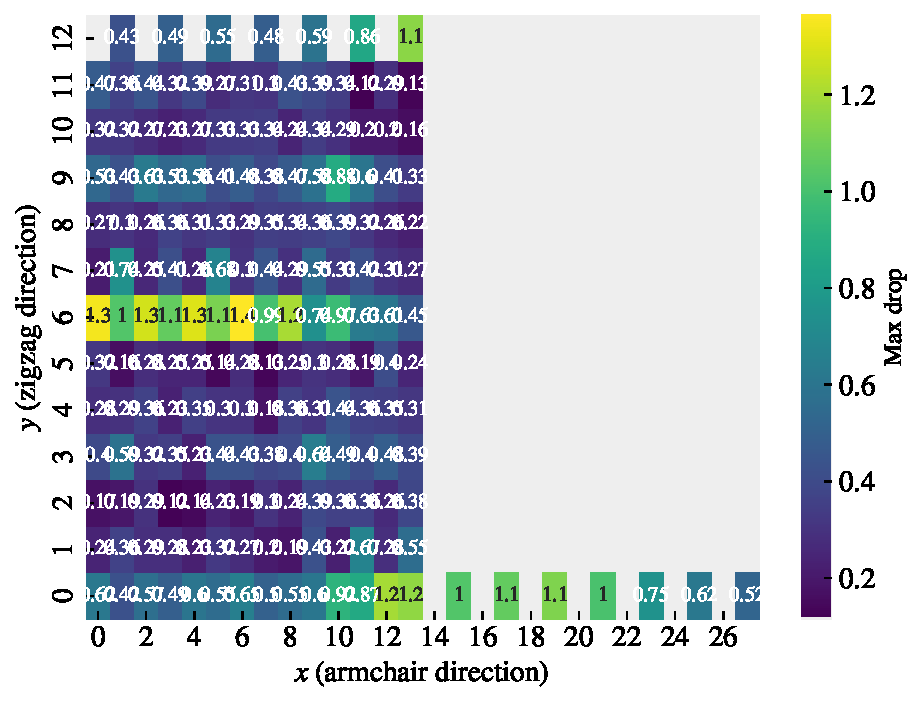
\includegraphics[width=\textwidth]{figures/search/ref_search_drop_hon_2_3_3_3_ref_search.pdf}
      \caption{Honeycomb $(2,3,3,3)$. (182)  Std = 0.27, Rel.\ Std = 0.60}
      % \label{fig:}
  \end{subfigure}
  \hfill
  \caption{\hl{CAPTION}}
  \label{fig:ref_search_top_data}
\end{figure}



\begin{figure}[H]
  \centering
  \includegraphics[width=\linewidth]{figures/search/RW_search_top5.pdf}
  \caption{RW search top results.}
  \label{fig:RW_search_top5}
\end{figure}  



\subsection{Genetic algorithm search}
The second approach to an accelerated search is through the genetic algorithm.
So far we have concluded that a minimization of the friction, with our system
specifications and model predictions, is not promising. Hence, we discard this
property for further study. We have also seen that the maximum style property
often shares similar top candidates, and thus we choose to only investigate the
max drop property, associated with the aim of creating a negative friction
coefficient. From the extended search, we have three candidates within the
Tetrahedron, Honeycomb and Random walk style. We use these three candidates as
the basis for an genetic agorithm search. We generate a population of 100
configurations using the settings associated with the top candidates. We run the
search for 50 generations as we did not see much difference for any longer
extensions. The Tetrahedron and Honeycomb search did not give any improvements
as the top configuration as the first generations was not improved on even
through the average score was rising. This was more or less the case for the
random walk as well with only a single new candidate giving a score of
\SI{0.300}{nN} for the drop property. The fact that starting from an existing
design did not give any useful results we attempted to start from a population
of random noise as well. We did with mixed porosities, even parts of $\{0.01,
0.05, 0.1, 0.2, 0.3\}$, and two for a porosity of 0.25 and 0.5 respectively.
This time the algorithm improved the top candidate throughout, but the actual
scores were disappointing. For the mixed porosity start, we found a top score of
\SI{0.299}{nN}. The top candidates did not seem to carry any higher order
patterns. To the human eye they still looked like random noise. By the use of
the gradient cam method \hl{not sure of name yet} we investigate for any
noticable patterns in the model. This is shown for the mixed porosity top
candidate in \cref{fig:GC_mixed_p} which can be compared to the top search
candidates in the drop category in figure \cref{fig:GC_pop_search}, \cref{fig:GC_hon_search} and \cref{fig:GC_RW_search}. While looking a such gradient visulizations can be mesmerizing they do not immediately reveal more about the underlying mechanisms. The ``attention'' of the model often matches well with the placement of the cuts, but it also reveals some frames where it seems consider the edge quite heavily. This especially relates to to the top and bottom edge which corresponds to the front and back of the sheet. Since these are also connected to the pull block it is really not an edge and thus it is a bit surprising if these should be of extra importance. Given the limited time resources we can follow up on these questions.



\begin{figure}[H]
  \centering
  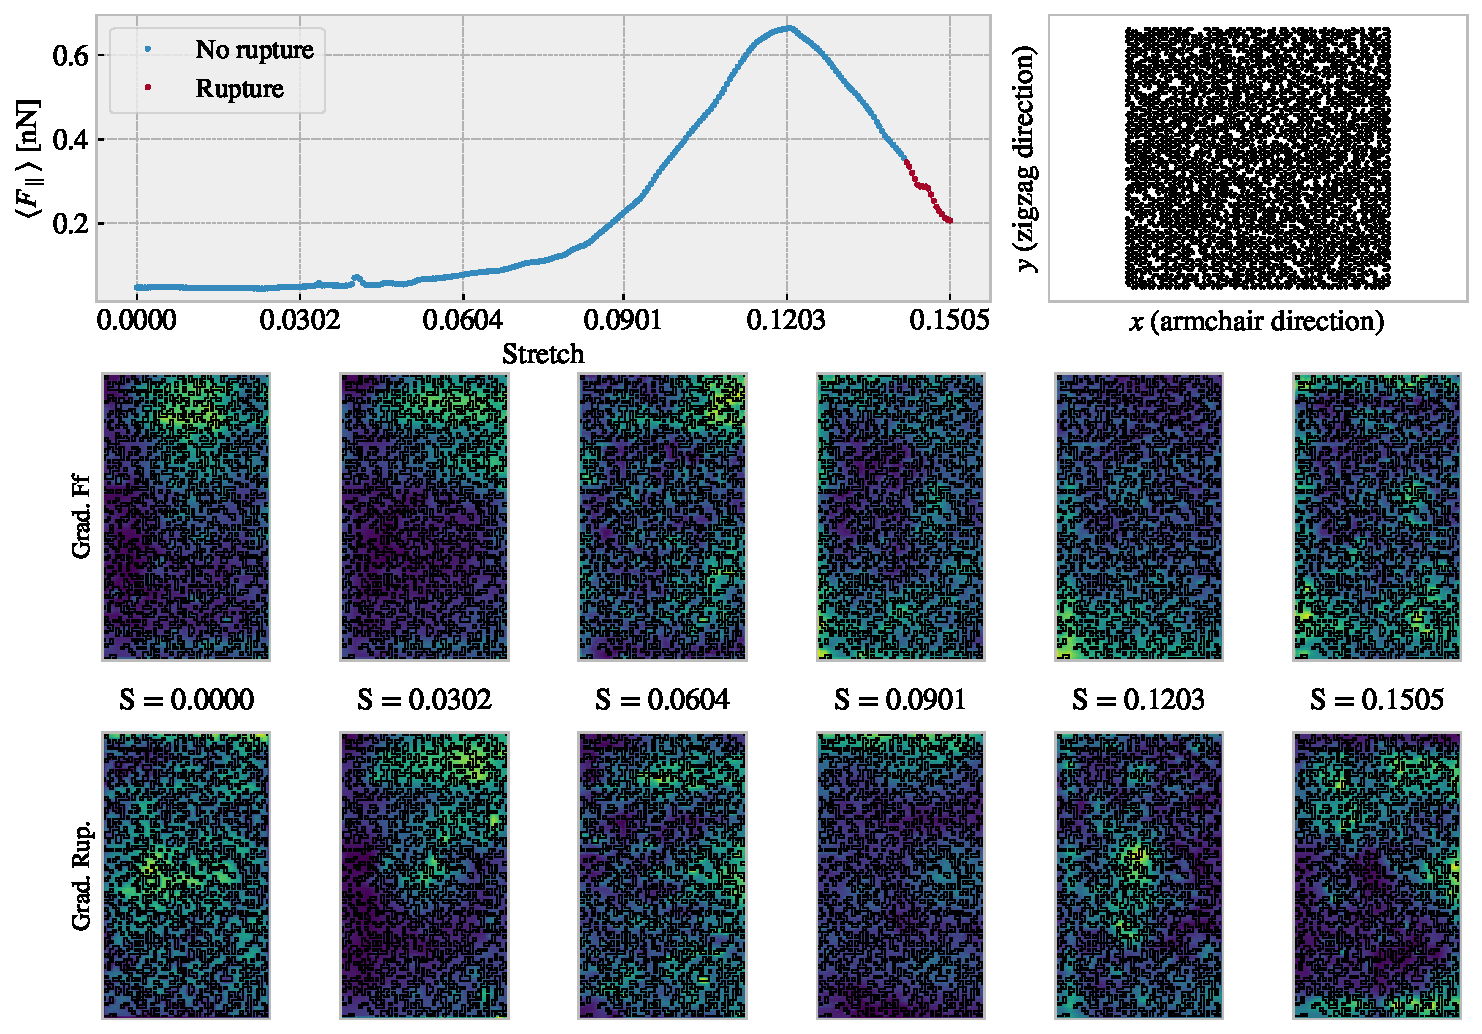
\includegraphics[width=0.8\linewidth]{figures/search/grad_cam_GA_RN_start_top0.pdf}
  \caption{$p \in \{0.01, 0.05, 0.1, 0.2, 0.3\}$.}
  \label{fig:GC_mixed_p}
\end{figure}  

\begin{figure}[H]
  \centering
  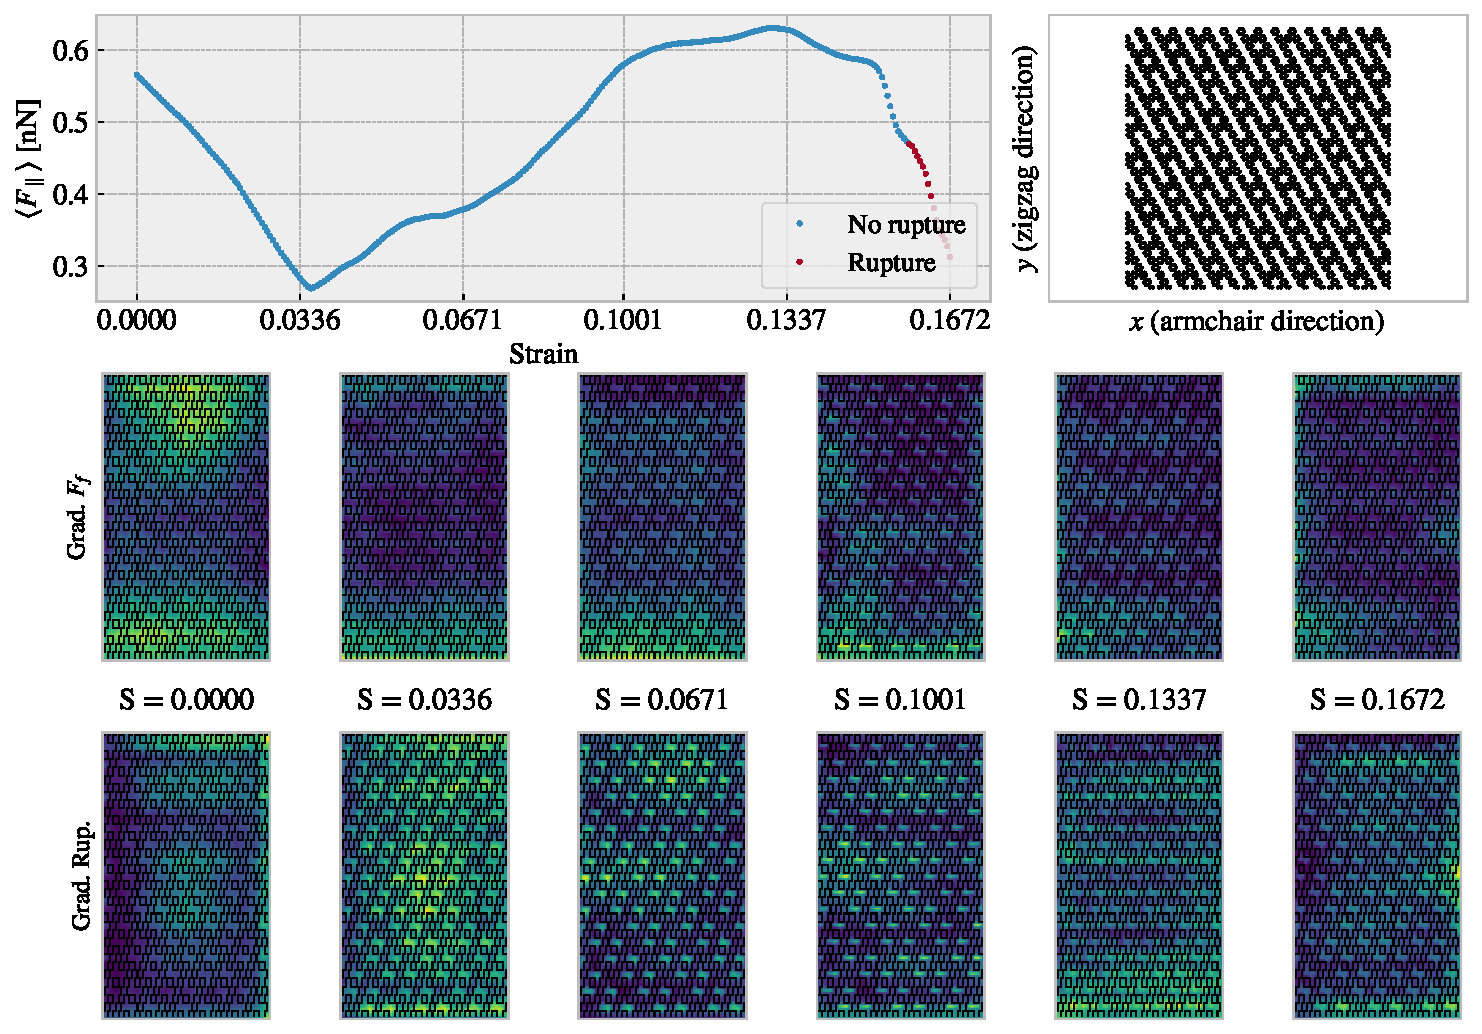
\includegraphics[width=0.8\linewidth]{figures/search/grad_cam_pop_1_7_1_1_4.pdf}
  \caption{Tetrahedron $(1,7,1)$, ref = $(1,4)$}
  \label{fig:GC_pop_search}
\end{figure}  


\begin{figure}[H]
  \centering
  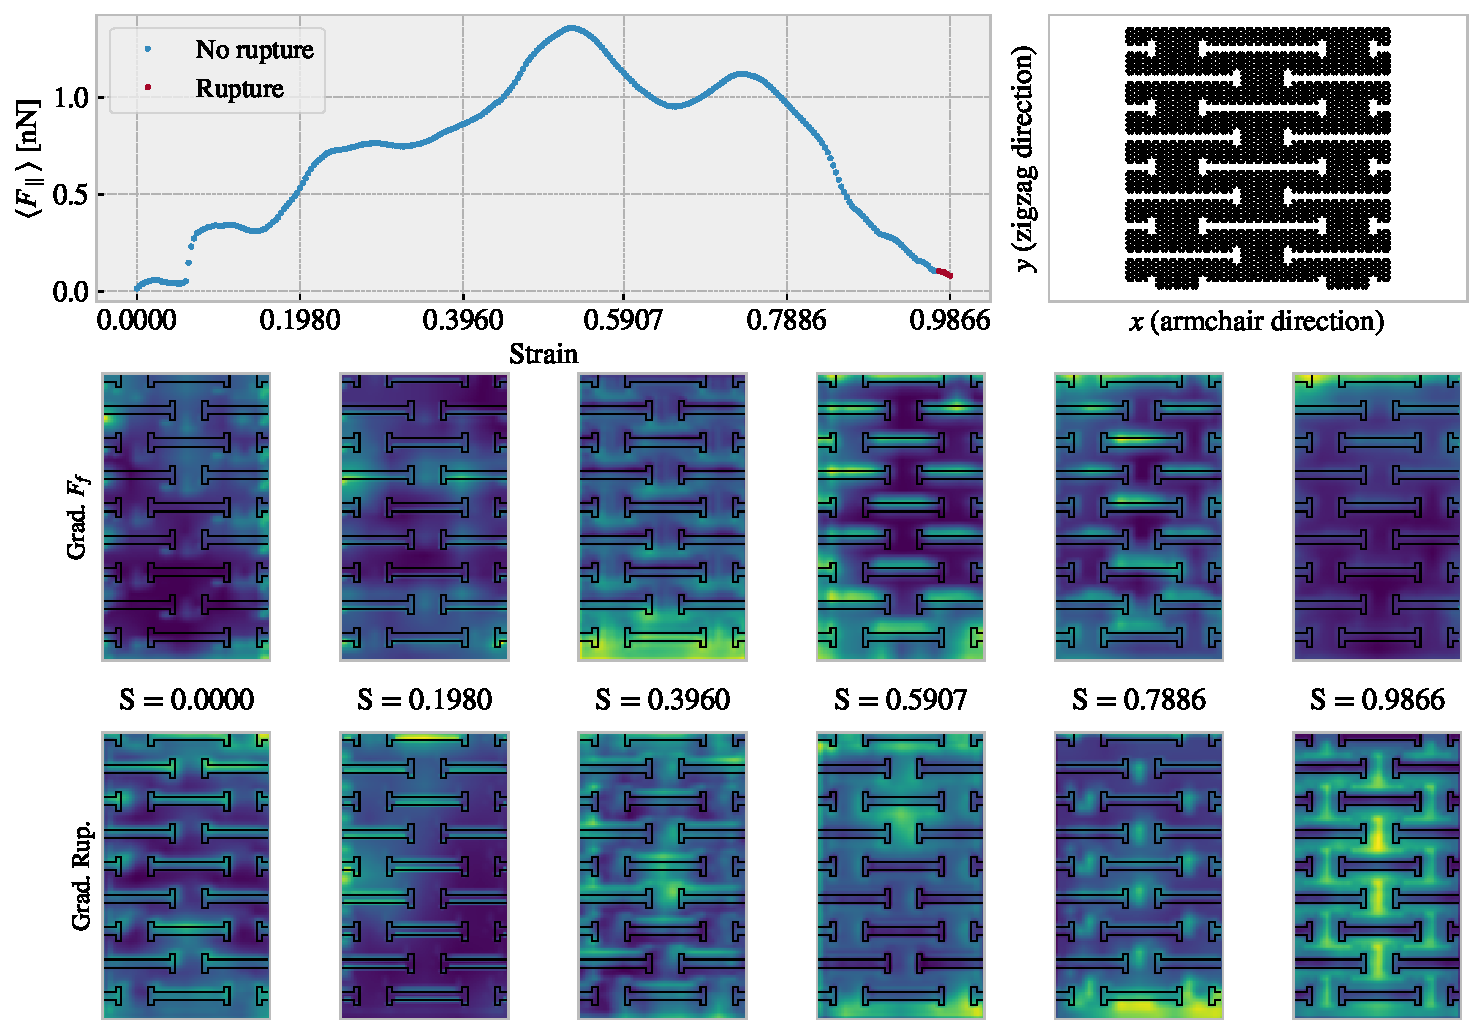
\includegraphics[width=0.8\linewidth]{figures/search/grad_cam_hon_3_3_5_3_12_0.pdf}
  \caption{Honeycomb $(3,3,5,3)$, ref = $(12,0)$}
  \label{fig:GC_hon_search}
\end{figure}  

\begin{figure}[H]
  \centering
  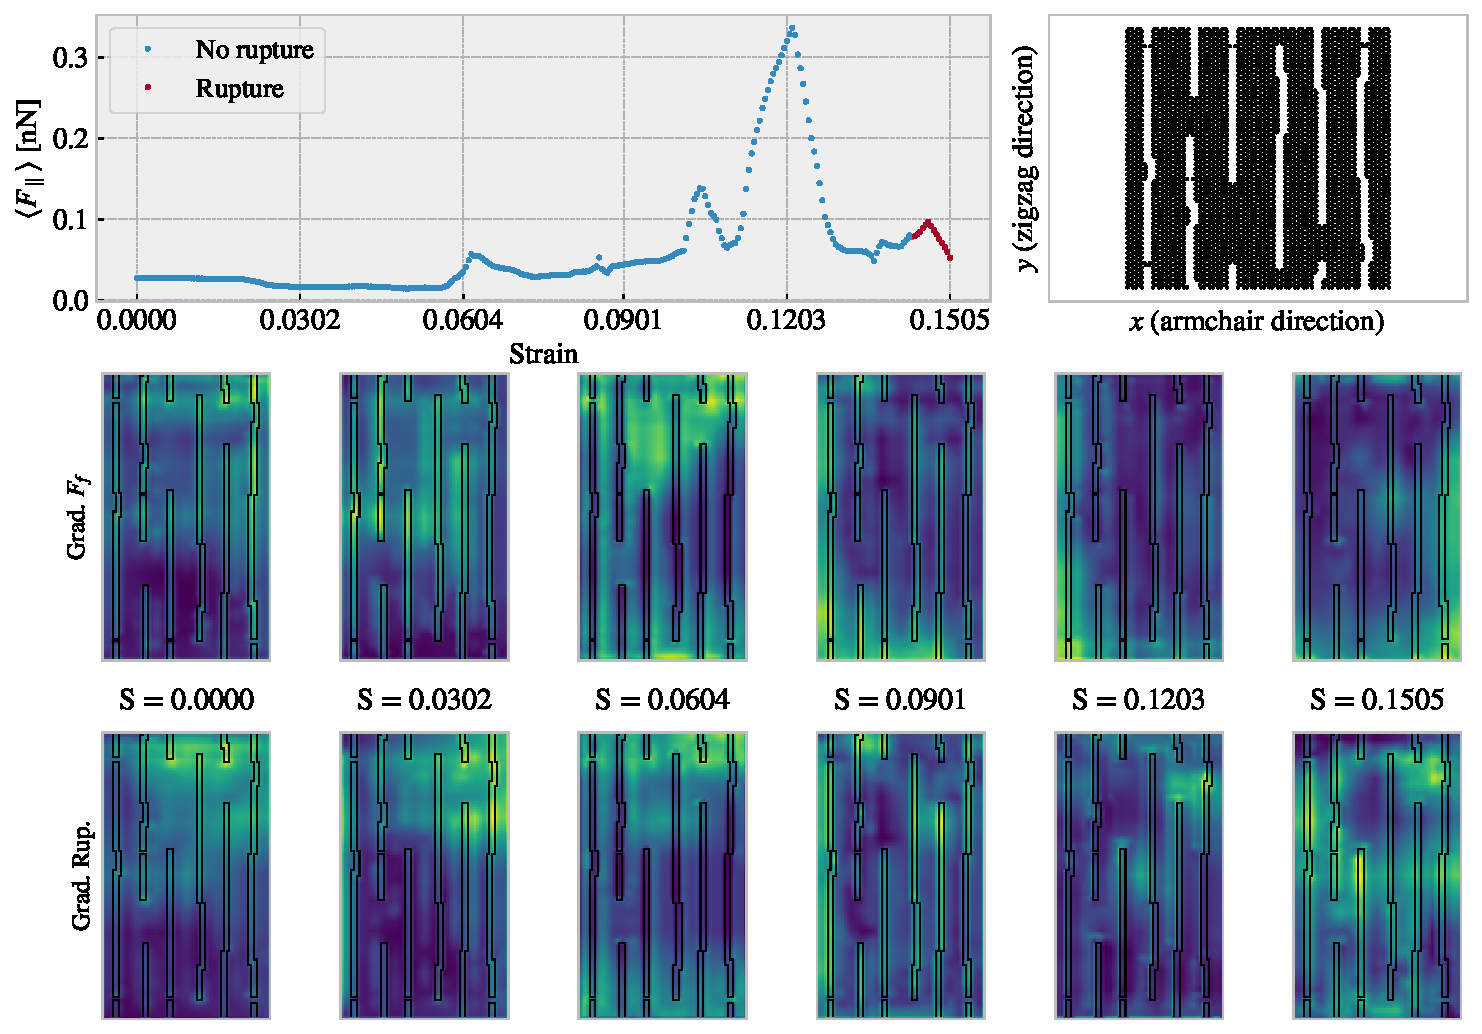
\includegraphics[width=0.8\linewidth]{figures/search/grad_cam_RW_search_max_drop0.pdf}
  \caption{RW.}
  \label{fig:GC_RW_search}
\end{figure}  




% The genetic algorithm approach could possible benefit for a consideration of 2D connections adn translation. It will force any positive patterns to be forced in their location and do not realize that making thoose repeatly will increase effect. It effectively sees every pixel like an unique gene and not really a positional property. 



